\chapter{Literature Review}\label{sec2_revisao_lit}
\section{Time Series Anomaly Detection}

In recent years, rapid technological advancements have led to a significant increase in the volume of data collected and generated from diverse sources such as sensors, databases, and files \cite{attoh2017big}. This large volume of data is now commonly referred to as Big Data. A substantial portion of Big Data consists of data points collected in sequential time steps, also known as time series. Analyzing time series data presents a complex set of challenges, such as: \cite{Tsai_Lai_Chao_Vasilakos_2015}. 

\begin{itemize}
    \item \textbf{Large Volume of Data}: Time series data can be collected at high frequencies, leading to large datasets that consume significant storage and processing resources.
    \item \textbf{High Dimensionality}: Data can be collected by multiple sensors, resulting in high-dimensional datasets, that, sometimes, can have multiple redundant variables.
    \item \textbf{Variables Correlations}: In multivariate time series, multiple variables might have complex correlations, making it challenging to model their relationships.
\end{itemize}

One of the most studied problems in this area is anomaly detection. It consists of identifying outliers or abnormal patterns within data and has a variety of applications, from financial systems and medical diagnosis to urban management and fault detection \cite{Samariya_Thakkar_2021}. 

The following sections will dive deeper into the concept of a time series, the different natures of anomalies in data, and some of the models used to detect these anomalies.

\subsection{Time Series}

A time series (TS) can be defined as a set of points indexed sequentially over time and is often divided into univariate and multivariate. A univariate TS is a set of real values from a single variable that changes over time $\textbf{X} = \{x_t\}$ for $t$ $\in$ $T$, where T is the total time. On the other hand, a multivariate TS is a set of real values from multiple variables that change over time, i.e., $\textbf{X} = \{\textbf{x}_t\}$ for $t$ $\in$ $T$, where $\textbf{x}_t$ is a k-dimensional vector defined by $\textbf{x}_t = (x_{1t}, ..., x_{kt})$ and each $x_{it}$ is a univariate TS. 

A subsequence of length $n \leq T$ can be defined as $\textbf{S} = \{\textbf{x}_{p:p+n}\}$ from the time series $\textbf{X}$, where $p \in T$ and $p \leq T-n+1$ \cite{Blazquez-Garcia_Conde_Mori_Lozano_2021}. 

Time series data exhibit dependencies that vary based on their type. In univariate time series, temporal dependency occurs when the value at time $t$, $x_t$, is influenced by its preceding values, $x_{p:t}$. In multivariate time series, in addition to temporal dependencies, there are spatial dependencies, representing the correlations between different variables within the same time step \cite{Zamanzadeh_Darban_Webb_Pan_Aggarwal_Salehi_2024}.

\subsection{Time Series Anomalies}

According to Grubbs \cite{Grubbs_1969} an anomaly can be defined as an outlier that deviates greatly from the general distribution of data. These outliers can be a single observation or a subsequence of the whole time series and they can be further distinguished as a local outlier, which deviates from the local behavior of the data, or a global outlier, which deviates from the global behavior of the data. Building on this, Blázquez-García et al. \cite{Blazquez-Garcia_Conde_Mori_Lozano_2021} divides anomalies into three main categories:

\begin{enumerate}
    \item \textit{Point Anomalies}: A point outlier can be defined as a single observation that deviates from the global behavior (global anomaly) or from the behavior of it's neighborhood (local anomaly). This type of anomaly can be identified using equation \ref{eq_point_anomaly}
    \begin{equation}
        |x_t - \hat{x}_t| > \tau
        \label{eq_point_anomaly}
    \end{equation}
    where $\hat{x}_t$ is the expected result, $x$ is the original data point and $\tau$ is the threshold. If the difference is greater than the threshold $\tau$, then $x_t$ is identified as an anomaly. Figure \ref{fig:point_anomaly} shows an example of this anomaly, where O1 is a local outlier and O2 is a global anomaly.

    \item \textit{Subsequence Anomaly}: A subsequence outlier refers to a consecutive portion of points from the time series whose joint behavior is abnormal. It is important to note that each of these data points alone doesn't need to be a point anomaly, but together they form an anomaly. Similarly to the point outliers, the subsequence outliers can be global or local. These anomalies can be identified by the equation \ref{eq_subsequence_anomaly}:
    \begin{equation}
        diss\left(C, \hat{C}\right) > \tau
        \label{eq_subsequence_anomaly}
    \end{equation}
    where $C$ is the the actual cycle or shape of the subsequence, $\hat{C}$ is the expected output, $\tau$ is the threshold and $diss$ is a function that computes the dissimilarity between the two subsequences, such as the cosine similarity. Figure \ref{fig:subsequence_anomaly} shows an example of this, where O1 is a local anomaly and O2 is a global anomaly.

    \item \textit{Time Series Anomaly}: A time series anomaly is an entire time series that presents unusual behavior. Note that this kind of anomaly can only be detected in multivariate time series, as it needs to consider the behavior of one feature compared to the others. Figure \ref{fig:Time_series_anomaly} shows an example of this problem, where Variable 4 behavior differs greatly from the other 3.
\end{enumerate}

%Darban et al. \cite{Zamanzadeh_Darban_Webb_Pan_Aggarwal_Salehi_2024} highlights another anomaly that can only occur in multivariate time series: the intermetric anomaly. An intermetric anomaly can be defined as an anomalous behavior in the correlation between two variables. Differently from the % An example of this is shown in Figure ?????.


\begin{figure}[H]
    \centering
    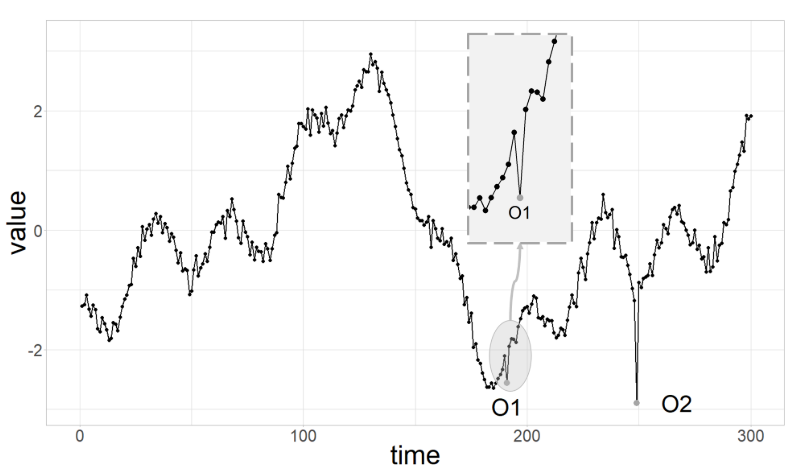
\includegraphics[width=10cm]{Cap2_LitReview/point_anomaly.png}
    \caption{Example of point anomalies in time series data, highlighting local (O1) and global outliers (O2) \cite{Blazquez-Garcia_Conde_Mori_Lozano_2021}.}
    \label{fig:point_anomaly}
\end{figure}

\begin{figure}[H]
    \centering
    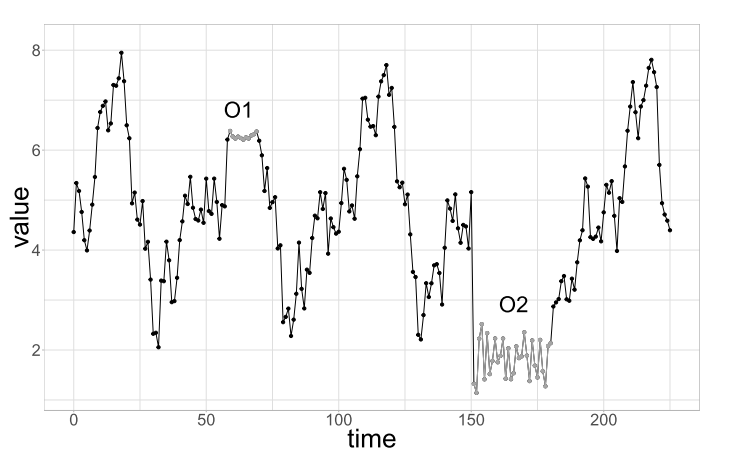
\includegraphics[width=10cm]{Cap2_LitReview/subseq_anomaly.png}
    \caption{Example of subsequence anomalies, showing local (O1) and global (O2) deviations in time series data \cite{Blazquez-Garcia_Conde_Mori_Lozano_2021}.}
    \label{fig:subsequence_anomaly}
\end{figure}

\begin{figure}[H]
    \centering
    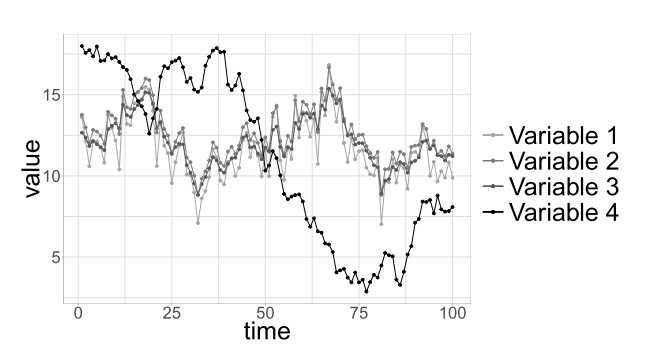
\includegraphics[width=10cm]{Cap2_LitReview/TS_anomaly.png}
    \caption{Example of a time series anomaly in a multivariate dataset, where Variable 4 significantly deviates from others \cite{Blazquez-Garcia_Conde_Mori_Lozano_2021}.}
    \label{fig:Time_series_anomaly}
\end{figure}

\section{Time Series Anomaly Detection Models} \label{sec-model-basics}

Since the 1960s, many models for anomaly detection have been proposed, ranging from statistical models to recent deep learning models. The common main idea behind all of those is to identify low probability, i.e. low density, regions, classifying points in those areas as anomalies \cite{Samariya_Thakkar_2021}. 

Statistical models use statistical tests, like the $\chi^2$ test, to identify abnormal points. Clustering-based models use cluster analysis to label anomalies, using, for example, the distance from the centroid of normal points or the number of points in a cluster. Distance-based models use the distance between the current time window and its neighborhood to classify anomalies. Density-based approaches use the density of the data points to find anomalies \cite{Samariya_Thakkar_2021}. These methods described above are called traditional methods.

In recent years, with the increase of computing power, deep learning models have become increasingly prominent in anomaly detection. Unlike the traditional methods, the main advantage of deep learning models is that they are capable of identifying complex temporal and spatial correlations between variables, especially in larger multidimensional datasets, without the need for a labeled dataset \cite{Choi_Yi_Park_Yoon_2021}. Darban et at. \cite{Zamanzadeh_Darban_Webb_Pan_Aggarwal_Salehi_2024} divides deep learning models into 3 main categories: forecasting-based models, reconstruction-based models, and representation-based models.

Forecasting-based models try to predict a future subsequence of the time series using historical data. These models learn the patterns and trends within data to anticipate what is expected to occur. Recurrent Neural Networks (RNNs) and Long Short-Term Memory (LSTMs) are examples of this category. Anomalous values are detected if they deviate greatly from what the model predicts.

Reconstruction-based models attempt to recreate the input timeseries based on the values of past points or windows. These models use architectures like autoencoders (AE) and Generative Adversarial Networks (GANs). Anomalies are identified using the reconstruction error between the predicted series and the original series. The advantage of reconstruction-based models over forecasting ones is that they adapt better to rapid changes in a timeseries, which may cause it to become unpredictable. This happens because reconstruction models have access to the current timeseries data, which is not available in forecasting models \cite{Zamanzadeh_Darban_Webb_Pan_Aggarwal_Salehi_2024}. This better precision comes with a delay in the detection time of an anomaly, but, in general, these models are preferred over forecasting models.

Representation-based models focus on learning meaningful representations of the data that can be used in downstream tasks, like anomaly detection.  These models use advanced architectures like transformers and self-supervised learning to extract high-level features from the data. From this representation, it is easier to solve a specific task and use simpler models (e.g., clustering or density-based methods) to identify anomalies. The downside of these models is that they are computationally expensive to train, often needing a large amount of data.

An important point to highlight is that the majority of the models described above are unsupervised models. An unsupervised model is a model that can learn patterns from data without the need for a labeled dataset. This flexibility is desired because of the inherently unlabeled nature of historical data and the unpredictability of anomalies, which makes it harder to define an anomaly, especially if anomalies are rare. In this work, the focus will be on unsupervised reconstruction models.

Another important point to note is that, as will be detailed in Sections \ref{sec-track-quality-accel} and \ref{sec-methodology}, the model proposed in this thesis is not designed specifically for anomaly detection. Instead, its primary objective is to learn how to reconstruct track irregularities from acceleration data. Despite that, the main idea that motivates the model's development is closely related to anomaly detection. For this reason, a review of anomaly detection methods was included.

\section{Basics of Deep Learning Models}

Before diving deeper into anomaly detection models, the fundamental concepts of deep learning will be presented first. This preliminary discussion will provide the necessary context and theoretical basis for the subsequent exploration of reconstruction models.

\subsection{Neural Networks} \label{sec-Neural_networks}

Neural networks are the most basic structure in deep learning. It is inspired by the way the human brain works \cite{AGATONOVICKUSTRIN2000717}. These networks are composed of thousands, or even millions, of interconnected units called perceptrons, which mimic the behavior of biological neurons. In a neural network, these perceptrons are arranged into multiple layers, as shown in Figure \ref{fig:neural_network-a}. In this illustration, each circle represents a single perceptron. 

The neural network is divided into three main components: 
\begin{itemize}
    \item The input layer: this layers receives raw data that will be precessed;
    \item The hidden layers: positioned between the input and output layers, these intermediate layers perform feature extraction;
    \item The output layer: this layer provides predictions or classifications
\end{itemize}

Each perceptron in a neural network processes input data linearly using the dot product. Given, then, an input array $\mathbf{x}$, the perceptron computes the output by multiplying $\mathbf{x}$ with an array of weights $\mathbf{w}$ and adding a bias $b$, producing a scalar output $o$ \cite{Gurney_1997}:
\begin{equation}
    o = \sum_{i}w_i x_i + b
\end{equation}

The weights and biases are learned and iteratively updated during the training process such that they minimize the errors.

However, in its basic form, a perceptron can only solve linearly separable problems. To address this limitation, modern perceptrons include an additional element: the activation function. An activation function introduces non-linearity into the model, enabling it to solve complex, non-linear problems \cite{Roth_2016}. For reasons that will be explained later, it is common to choose differentiable activation functions. Common activation functions include the Rectified Linear Unit (ReLU) and the hyperbolic tangent (tanh). The general structure of a perceptron, including the activation function, is illustrated in Figure \ref{fig:neural_network-b}.

%\begin{figure}[H]
 %   \centering
  %  \includegraphics[width=0.5\linewidth]{Cap2_LitReview/model_basics/Colored_neural_network.png}
   % \caption{\cite{enwiki:1294206888}}
    %\label{fig:neural_network}
%\end{figure}

\begin{figure}[H]
    \centering
    \begin{subfigure}{0.45\textwidth}
        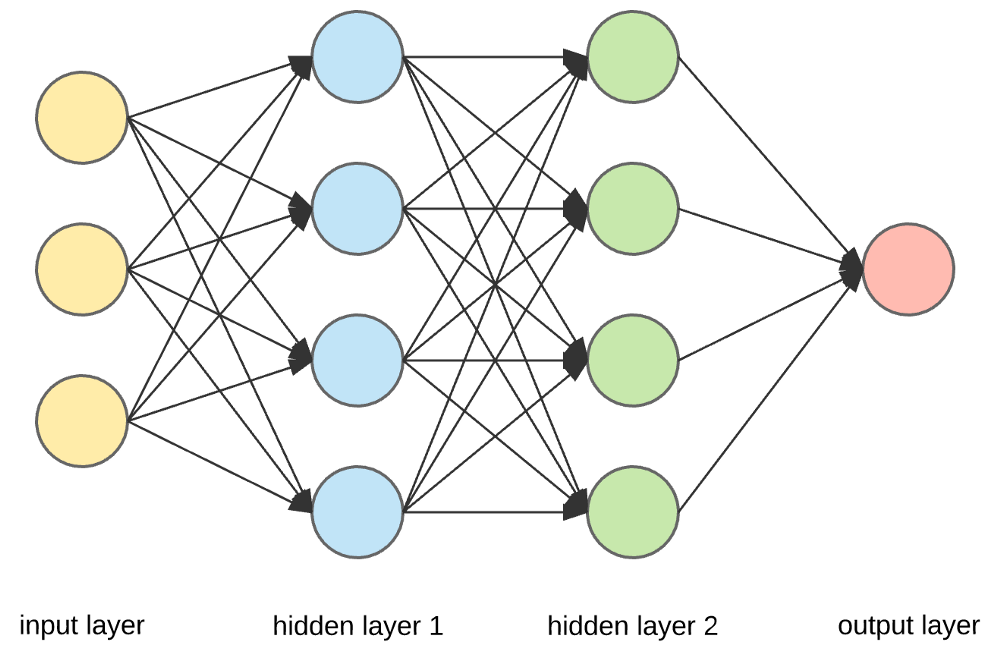
\includegraphics[width=7cm]{Cap2_LitReview/model_basics/Neural_networks/neural_network.png}
        \caption{}
        \label{fig:neural_network-a}
    \end{subfigure}
    \hspace{0.2cm}
    \begin{subfigure}{0.45\textwidth}
        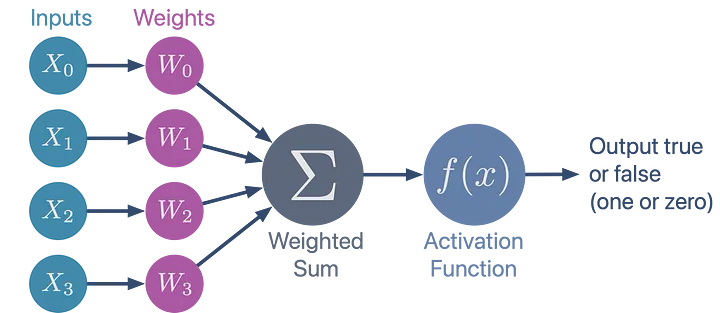
\includegraphics[width=8cm]{Cap2_LitReview/model_basics/Neural_networks/perceptron.png}
        \caption{}
        \label{fig:neural_network-b}
    \end{subfigure}
    \caption{Structure of a neural network. $\boldsymbol{(a)}$ Fully connected perceptrons arranged in layers \cite{P._2025}. $\boldsymbol{(b)}$ Perceptron with activation function \cite{Weaver_2024}.}
    \label{fig:neural_network}
\end{figure}

As mentioned earlier, the weights and biases of the perceptrons are adjusted and optimized during the training phase of a neural network. This optimization process involves a method called backpropagation, which is essential for minimizing the error in predictions. Backpropagation, discussed in detail in Section \ref{sec-backpropagation}, leverages the gradient descent algorithm to iteratively update the network's parameters, ensuring improved accuracy over successive training iterations.

\subsection{Backpropagation} \label{sec-backpropagation}

During the training phase of a neural network, its weights and biases are systematically optimized to minimize the error. This iterative process comprises two key subprocesses: a forward pass followed by a backward pass. In a forward pass, the inputs are passed through the network and the outputs are calculated. Then, given an expected output, an error is computed using a function called the loss function. The backward pass, then, uses this error to update the weights and biases of the neural network, making it better at making right predictions. This process continues until the error is small enough.

The process of propagating the error back through the network during the backward pass is referred to as backpropagation. It can be broken down into four primary steps \cite{cilimkovic2015neural}:

\begin{enumerate}
    \item Feed foward the inputs;
    \item Backpropagation to the output layer;
    \item Backpropagation to the hidden layers;
    \item Weights updates.
\end{enumerate}

The first step is just feeding forward the inputs $\mathbf{x}$ through the network and obtaining the outputs $\mathbf{o}$. Then, a loss is computed using the loss function $\mathbf{L}$. There are a variety of loss functions, an example being the Mean Squared Error (MSE):
\begin{equation}
    \mathbf{L} = \frac{1}{N} \sum_{i} \left(y_i-o_i\right)^2
\end{equation}
where $y_i$ is the desired output and $o_i$ is the network output. To backpropagate the error, the algorithm computes gradients of the loss function with respect to the parameters of the neural network. This is done using the chain rule twice \cite{Roth_2016}:
\begin{equation}
    \frac{\partial \mathbf{L}}{\partial w_{ij}} = \frac{\partial \mathbf{L}}{\partial o_j}
    \frac{\partial o_j}{\partial net_j}\frac{\partial net_j}{\partial w_{ij}}
\end{equation}
where $w_{ij}$ is the i-th weight of the j-th perceptron, $net_j$ is the result of the dot product before applying the activation function, i.e.,
\begin{equation}
    net_j = \sum_i w_{ij} x_j
\end{equation}
with $x_j$ being the input, and $o_j$ the perceptron output, i.e.,
\begin{equation}
    o_j = \varphi (net_j)    
\end{equation}
where $\varphi$ is the activation function of the perceptron. For this reason, it is necessary that the activation function is a differentiable function. 

To update the weights, the algorithm computes, then, the incremental $\Delta w_{ij}$ using:
\begin{equation}
    \Delta w_{ij} = -\eta \delta_j x_{ij}
\end{equation}
where $\eta$ is a small positive number known as the learning rate, $\delta_j = \frac{\partial \mathbf{L}}{\partial net_j}$ and $x_{ij}$ are the inputs of the j-th perceptron. 

The weights are updated as:
\begin{equation}
    w_{ij} \xleftarrow{} w_{ij} + \Delta w_{ij}
\end{equation}
For a full demonstration of these formulas, check Roth \cite{Roth_2016}. 

Despite its effectiveness, the classical backpropagation algorithm has some problems associated with its convergence. For example, if the learning rate is too small, the convergence is very slow and can converge to a local minimum; on the other hand, if it is too large, the algorithm can diverge \cite{ruder2016overview}. Several modifications to the original algorithm have been proposed. In Rumelhart et al. \cite{Rumelhart_Hinton_Williams_1986} authors propose to include a momentum term to speed up the convergence. In Tieleman \cite{1370017282431050757} the author proposes an adaptative learning rate algorithm that divides the learning rate by the moving average of the gradients. Additionally, Kingma and Ba \cite{kingma2017adammethodstochasticoptimization} introduced the Adam optimizer, adapting the learning rate for each parameter individually.

\subsection{Convolutional Neural Networks} \label{section-CNN}
%Escrever sobre treinamento, dps backpropagation e adam, CNN, LSTM, transformers.
Convolutional neural networks (CNN) achieved great popularity in modern machine learning, after Krizhevsky, Sutskever and Hinton \cite{NIPS2012_c399862d} paper. In this work, the authors proposed a deep CNN that won the ImageNet LSVRC-2010 contest, outperforming second place by a large margin. 

A CNN, similarly to the neural network, was inspired by the biological neurons, but, different from the conventional neural network, where all the neurons are connected and interact with all neurons in adjacent layers, the CNN employs a sparse architecture, i.e., the neurons are connected only to a local region of the input. This sparsity reduces the amount of training parameters, which reduces the computational cost and speeds up the training process \cite{Alzubaidi_Zhang_Humaidi_Al_Dujaili_Duan_Al_Shamma_Santamaria_Fadhel_Al_Amidie_Farhan_2021, 9451544}. 

CNNs are widely used in computer vision to process and analyze 2D images and are used to solve a variety of image-related problems, like classification and object detection. While this section focuses on explaining CNN concepts with the assumption of a 2D input, it is important to note that the principles discussed are equally applicable to 1D inputs, like in a timeseries.

The basic block of a CNN is the convolution operation. A convolution can be defined as the dot product between an input $x$ of shape $(m,m,r)$, where $m$ is the height, which is the same as the width, and $r$ is the depth, also called the channel number, and $k$ convolutional filters, called kernels. A kernel is a grid of weights, with shape $(n,n, q)$, where $n < m$ and $q \leq r$, that convolves with the input, producing, each, an output of size $(m-n-1)$, called the feature maps \cite{Alzubaidi_Zhang_Humaidi_Al_Dujaili_Duan_Al_Shamma_Santamaria_Fadhel_Al_Amidie_Farhan_2021}. These kernels compute the pass value similarly to the 
\begin{equation}
    h^k = f\left(W^k * x + b_k\right)
\end{equation}

where $W^k$ is the vector of weights from the kernel, $f$ is an activation function, and $b^k$ is the bias. Figure \ref{fig:conv-example} shows an example of this operation between a 2D binary matrix and a $3\times3$ kernel. 

\begin{figure}[H]
    \centering
    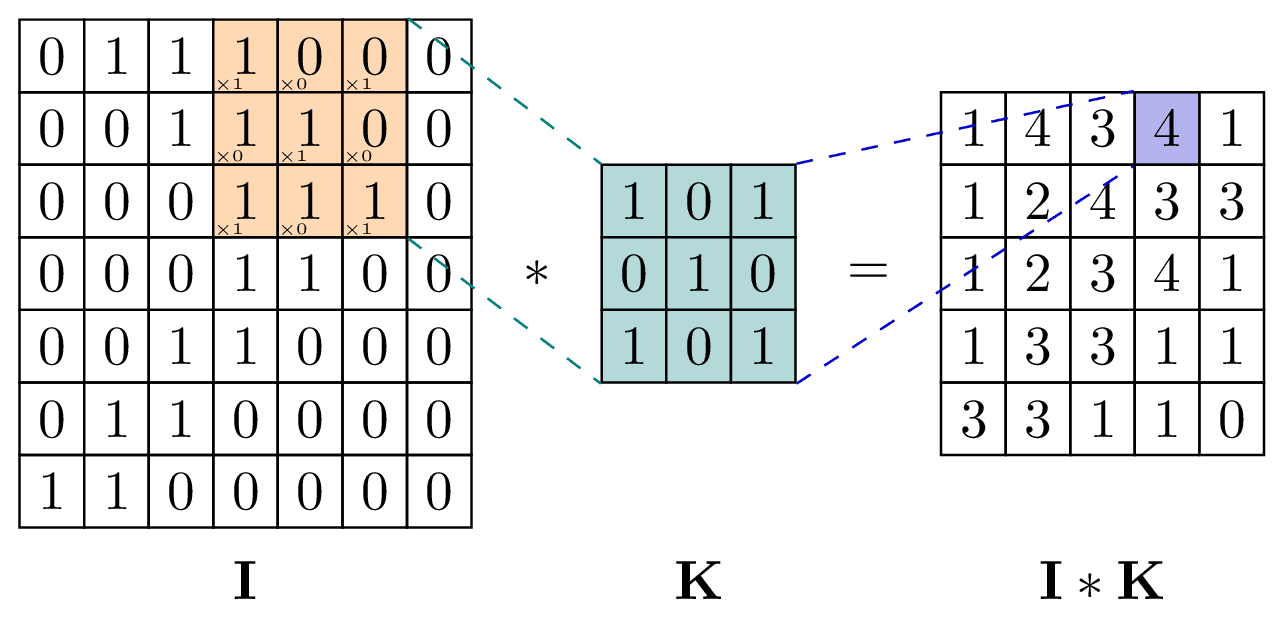
\includegraphics[width=9cm]{Cap2_LitReview/model_basics/Convolutional_NN/conv2d.png}
    \caption{Illustration of the convolution operation in a convolutional neural network. \cite{Riebesell_2022}}
    \label{fig:conv-example}
\end{figure}

In addition to the convolution operation, there are two other important parameters in convolutional neural networks: the padding and the stride. Their main function is to control the output size of the convolution, helping to maintain the spatial characteristics of the input. 

The padding is the process of adding additional rows and columns around the border of the input matrix, typically filled with zeros, a process known as zero padding. Without the padding, a convolution with a kernel of size $n\times n$ reduces the output size by $n-1$ in each spatial dimension. This would cause a rapid decrease in the size of the features, that would force the use of small kernels \cite{Goodfellow_Bengio_Courville_2018}.

Stride, on the other hand, controls how the kernel moves across the input matrix, by skipping some of the elements from it. In a stride 1 convolution, the kernel shifts one unit at a time, covering all the positions. In a stride 2 convolution, the kernel would shift 2 elements each time, which causes the kernel to convolve with every other element. In general, a stride of size $s$ means that the kernel will only convolve every $s$ elements. This is done primarily to reduce computational cost, at the expense of extracting the features less finely \cite{Goodfellow_Bengio_Courville_2018}. 

Now with these two additional operations, the output size can be computed using the formula:
\begin{equation}
    O = \left\lfloor \frac{I + 2 \cdot p - k}{s} \right\rfloor + 1
    \label{eq:conv_output}
\end{equation}
where $O$ is the output size, $I$ is the input size, $p$ is the padding, $k$ is the kernel size, and $s$ is the stride.

Another important feature that is widely used in CNNs is the pooling layer. Pooling layers are used to further reduce the spatial dimension of the feature map by replacing the output value of the convolution operation with a local summary statistic, which helps the model to develop representations that are invariant to small translations \cite{Goodfellow_Bengio_Courville_2018}. 

One of the most widely used types is max pooling, which selects the maximum value within a local neighborhood, as shown in Figure \ref{fig:pooling-example}. Other common pooling methods include average pooling, which computes the mean of the values within the region, and weighted average pooling, where each value contributes proportionally based on predefined weights.

\begin{figure}[H]
    \centering
    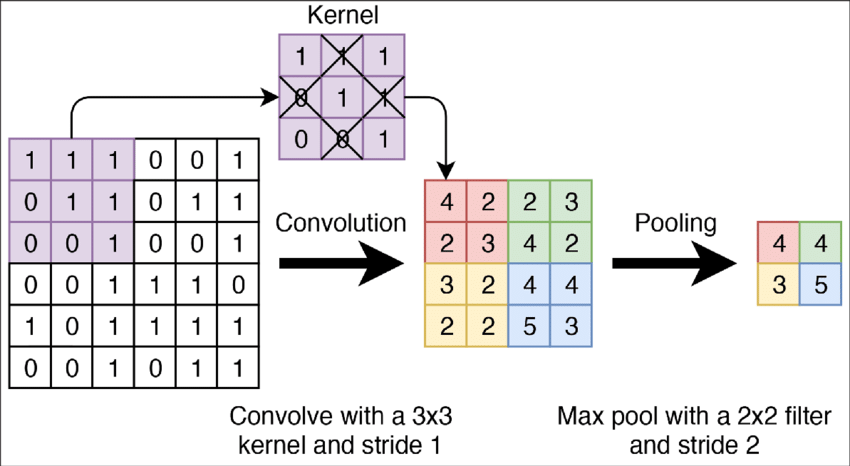
\includegraphics[width=9cm]{Cap2_LitReview/model_basics/Convolutional_NN/Schematic-representation-of-a-convolution-and-pooling-layer-in-a-CNN.png}
    \caption{Example of max pooling operation in a convolutional neural network. \cite{Verschoof-van}}
    \label{fig:pooling-example}
\end{figure}

\subsection{Recurrent Neural Networks} \label{section-RNN}

Recurrent Neural Networks (RNNs) are a type of artificial neural network specifically designed to work with sequential data, such as time series, speech recognition, text generation, and language modeling \cite{fang-wei,Alzubaidi_Zhang_Humaidi_Al_Dujaili_Duan_Al_Shamma_Santamaria_Fadhel_Al_Amidie_Farhan_2021}. The main difference between an RNN and the networks discussed in Sections \ref{sec-Neural_networks} and \ref{section-CNN} is how data is processed inside the RNN. In the MLP and the CNN networks, it is assumed that each input is independent from each other, which can be a valid assumption when dealing with images, but might be a severe limitation when dealing with sequential data, like weather data, where, for example, the current temperature depends on the last few measurements.

RNNs deal with this kind of problem by introducing a cycle in their architecture  allows information to persist across time steps \cite{schmidt2019recurrentneuralnetworksrnns}, as shown in Figure \ref{fig:RNN-struct}. The key idea is to add a hidden-to-hidden weight matrix $\boldsymbol{W}_{hh}$ that carries information from the previous hidden state $\boldsymbol{H}_{t-1}$ in the computation of the current hidden state $\boldsymbol{H}_t$. 

The current hidden state can be computed using Equation \ref{eq-RNN-hidden}:
\begin{equation}
    \boldsymbol{H}_t = \phi(\boldsymbol{X}_t \boldsymbol{W}_{xh} + \boldsymbol{H}_{t-1} \boldsymbol{W}_{hh} + \boldsymbol{b}_h)
    \label{eq-RNN-hidden}
\end{equation}
where $\boldsymbol{X}_t$ is the input vector, $\boldsymbol{W}_{xh}$ is the input-to-hidden weight matrix, $\boldsymbol{b}_h$ is the bias, and $\phi$ is an activation function. 

An important observation is that it is not necessary to explicitly include all previous hidden states, from $\boldsymbol{H}_{0}$ up to $\boldsymbol{H}_{t-2}$, when computing $\boldsymbol{H}_t$. This is because, at each iteration, the RNN updates $\boldsymbol{H}_{t}$ by combining the input $\boldsymbol{X}_t$ with the previous hidden state $\boldsymbol{H}_{t-1}$, which is the result of the computation between $\boldsymbol{X}_{t-1}$ and $\boldsymbol{H}_{t-2}$, and so on recursively. This way, the network can keep information about the previous time steps when computing the next one.

\begin{figure}[H]
    \centering
    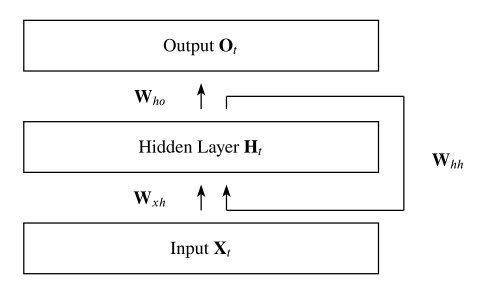
\includegraphics[width=9cm]{Cap2_LitReview/model_basics/RNN/rnn.png}
    \caption{Architecture of a recurrent neural network showing the recurrent connections between hidden states. Adapted from \cite{schmidt2019recurrentneuralnetworksrnns}}
    \label{fig:RNN-struct}
\end{figure}

The main problem in the original RNN architecture arises during the training phase, specifically when computing gradients for weight updates. As gradients are propagated backward through time, a series of repeated multiplications occurs. If these values are greater than 1, the gradients can grow exponentially, causing the network weights to change abruptly fast. Conversely, if the values are less than 1, the gradients decay exponentially, which causes the gradient to vanish \cite{kolen,pmlr-v9-glorot10a}. The vanishing gradient then causes the network to forget information from the initial time steps, which makes it difficult for RNNs to learn long-term dependencies in data.

This inherent problem motivated the introduction of more complex architectures, such as the LSTM networks. These networks will be explained in more detail in \ref{sec-LSTM}, but they mitigate the vanishing gradient problem, which caused the original RNNs to be barely used in today's research \cite{fang-wei,GAO2019279}.

\subsection{LSTM} \label{sec-LSTM}

Long Short-Term Memory (LSTM) units were introduced by Hochreiter and Schmidhuber in 1997 \cite{Hochreiter} and were specifically designed to deal with the vanishing gradient problem. Differently from vanilla RNNs described in Section \ref{section-RNN}, which struggle to retain information over long sequences, LSTM cells are specifically designed to capture long-term dependencies by preserving information across many time steps \cite{ALSELWI2024102068}.

The core idea behind the LSTM architecture lies in its gating mechanism, which regulates the flow of information through the cell. This mechanism is composed of three gates: the forget gate, the input gate, and the output gate, shown in Figure \ref{fig:LSTM-struct}. Each gate uses a sigmoid activation function, producing values between 0 and 1 to determine how much information should pass through \cite{schmidt2019recurrentneuralnetworksrnns}.

\begin{itemize}
    \item The forget gate decides which parts of the previous cell state should be discarded, allowing the network to “forget” irrelevant or outdated information. 
    \item The input gate determines which portions of the new input information should be added to the cell state.
    \item The output gate controls which parts of the internal cell state are exposed as the output hidden state at the current time step.
\end{itemize}

The forget and input gates are responsible for updating the cell state, which acts as an internal memory, carrying forward important information throughout the sequence. The output gate, meanwhile, regulates how much of the updated cell state should influence the hidden state output. Through this mechanism, LSTMs are able to maintain and regulate long-term information flow \cite{ALSELWI2024102068}.

\begin{figure}[H]
    \centering
    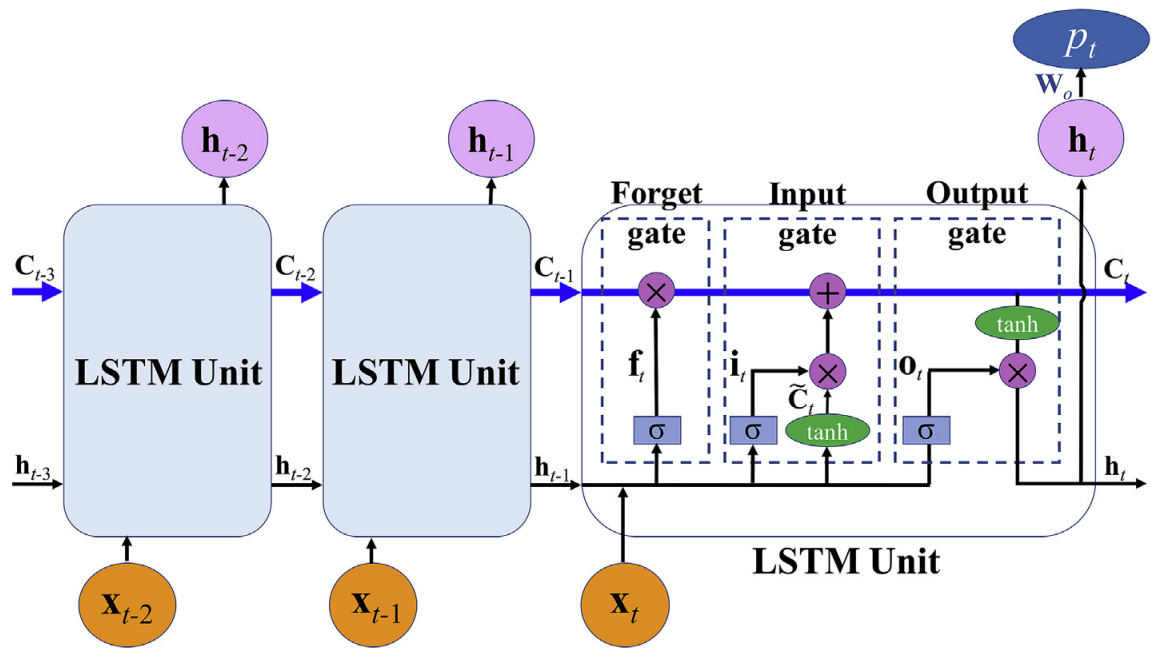
\includegraphics[width=9cm]{Cap2_LitReview/model_basics/LSTM/LSTM_Arch.png}
    \caption{Structure of an LSTM cell with input, forget, and output gates. Adapted from \cite{WEI2021453}}
    \label{fig:LSTM-struct}
\end{figure}

The LSTM unit can be mathematically described as follows. Given an input vector $\boldsymbol{X}_t$ at time step $t$ and the previous hidden state $\boldsymbol{h}_{t-1}$, the LSTM computes the output gate $\boldsymbol{o}_t$, the input gate $\boldsymbol{i}_t$, and the forget gate $\boldsymbol{f}_t$ using the following equations:
\begin{equation}
    \boldsymbol{o}_t = \sigma\left(\boldsymbol{X}_t \boldsymbol{W}_{xo} + \boldsymbol{h}_{t-1}\boldsymbol{W}_{ho} + \boldsymbol{b}_o\right)
    \label{eq-LSTM-Ot}
\end{equation}
\begin{equation}
    \boldsymbol{i}_t = \sigma\left(\boldsymbol{X}_t \boldsymbol{W}_{xi} + \boldsymbol{h}_{t-1}\boldsymbol{W}_{hi} + \boldsymbol{b}_i\right)
    \label{eq-LSTM-It}
\end{equation}
\begin{equation}
    \boldsymbol{f}_t = \sigma\left(\boldsymbol{X}_t \boldsymbol{W}_{xf} + \boldsymbol{h}_{t-1}\boldsymbol{W}_{hf} + \boldsymbol{b}_f\right)
    \label{eq-LSTM-Ft}
\end{equation}
After this computation, the LSTM unit computes the candidate memory cell $\boldsymbol{\tilde{C}}_t$, which represents the candidate information that could be added to the cell state, as:
\begin{equation}
    \boldsymbol{\tilde{C}}_t = \tanh \left(\boldsymbol{X}_t \boldsymbol{W}_{xc} + \boldsymbol{h}_{t-1}\boldsymbol{W}_{hc} + \boldsymbol{b}_c\right)
    \label{eq-CNN-Candidate}
\end{equation}

After that, the LSTM introduces the previous memory content $\boldsymbol{C}_{t-1}$, which, together with the other gates, controls how much of the old memory information will be retained in the new memory state $\boldsymbol{C}_{t}$, which can be computed using: 
\begin{equation}
    \boldsymbol{C}_t = \boldsymbol{f}_t \otimes \boldsymbol{C}_{t-1} + \boldsymbol{i}_t \otimes \boldsymbol{\tilde{C}}_t
\end{equation}
where $\otimes$ denotes the element-wise multiplication. Finally, the LSTM unit computes the hidden state $\boldsymbol{h}_t$ as:
\begin{equation}
    \boldsymbol{h}_t = \boldsymbol{o}_t \otimes \tanh (\boldsymbol{C}_t)
\end{equation}

It is important to notice the hidden state $\boldsymbol{h}_t$ is used as the output of the LSTM cell and, together with the memory state $\boldsymbol{C}_t$, is used in the computation of the next time step.

\subsection{Attention} \label{sec-attention}

Attention is an important concept in deep learning that was first introduced by Bahdamau, Cho and Bengio \cite{bahdanau2016neuralmachinetranslationjointly} in a machine translation problem and gained widespread popularity with the famous paper "Attention Is All You Need" proposed by Vaswani et al. \cite{vaswani2023attentionneed}, where the authors proposed the transformer architecture. Inspired by the human attention of selectively focusing on relevant information, attention mechanisms enable neural networks to assign different weights to different parts of the input, allowing the model to concentrate on the most important elements of the data. This selective focus not only improves the model's interpretability but also makes it possible to handle large amounts of information more efficiently, reducing computational overhead \cite{NIU202148}.

The attention mechanism works by taking a vector of features $\boldsymbol{F}$, which are obtained after the input data $\boldsymbol{X}$ is passed through a feature extraction model to extract the feature vectors $\boldsymbol{f}_1$, to $\boldsymbol{f}_n$. This feature extractor can vary depending on the task and, in the case of time series analysis, for example, it could be an encoder composed of CNNs, MLPs, or LSTMs, that produces the latent representations $\boldsymbol{f}_1$ to $\boldsymbol{f}_n$ \cite{Brauwers_2023}.

From the feature vectors $\boldsymbol{F}$ the model then extracts the key and value vectors $\boldsymbol{K}$ and $\boldsymbol{V}$, respectively. These vectors are usually obtained through a linear transformation of $\boldsymbol{F}$ using the weight matrix $\boldsymbol{W}_K$ and $\boldsymbol{W}_V$.

After that, the model introduces a query vector $\boldsymbol{Q}$, which is a task-specific vector that guides the attention mechanism to focus on the most important vectors \cite{Brauwers_2023,NIU202148}. From the query and key vectors, the model then computes the energy score $\boldsymbol{e}$ using a score function $f$:
\begin{equation}
    \boldsymbol{e} = f\left(\boldsymbol{Q},\boldsymbol{K}\right)
\end{equation}
where $f$ can be a variety of functions, such as the scaled dot product \cite{vaswani2023attentionneed}:
\begin{equation}
    f\left(\boldsymbol{Q},\boldsymbol{K}\right) = \frac{\boldsymbol{Q}^T \boldsymbol{K}}{\sqrt{d_k}}
\end{equation}

The energy scores $\boldsymbol{e}$ are then mapped to the attention weights $\boldsymbol{\alpha}$ using an attention distribution function $\mathrm{g}$, usually the softmax function \cite{NIU202148}:
\begin{equation}
    \boldsymbol{\alpha} = \mathrm{g}(\boldsymbol{e})
\end{equation}

Using the attention weights $\boldsymbol{\alpha}$ and the value vector $\boldsymbol{V}$, the model computes the context vector $\boldsymbol{c}$ using:
\begin{equation}
    \boldsymbol{c} = \sum_{l=1}^{n} \alpha_l \boldsymbol{V}_l  
\end{equation}
where $\alpha_l \in \mathrm{R}^1$ is the weight of the l-th vector. Figure \ref{fig:Attention-struct} shows the architecture of the attention model.

\begin{figure}[H]
    \centering
    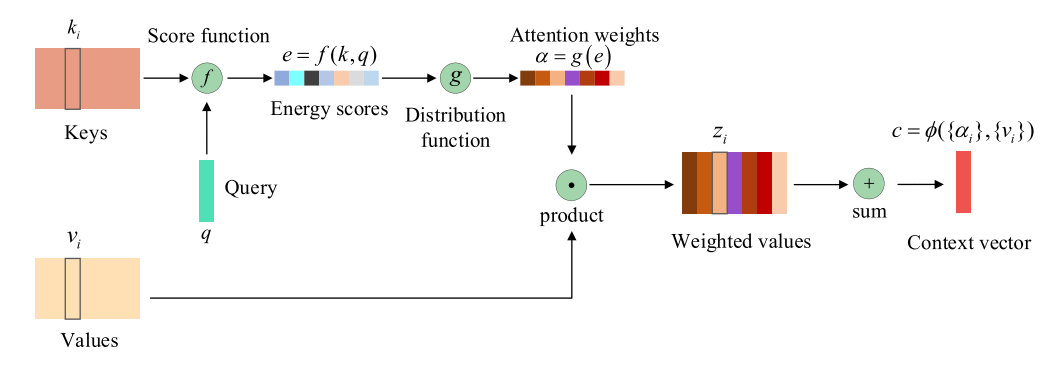
\includegraphics[width=12cm]{Cap2_LitReview/model_basics/Attention/attention-struct.png}
    \caption{Diagram of the attention mechanism showing query, key, value vectors, and the computation of the context vector. \cite{NIU202148}}
    \label{fig:Attention-struct}
\end{figure}

\subsection{Transformers}

The transformer architecture was introduced by Vaswani et al. \cite{vaswani2023attentionneed} and, since then, has gained widespread popularity in various fields, such as natural language processing (NLP), computer vision (CV) and time series analysis \cite{lin2021surveytransformers}. It is built upon the attention mechanism, shown in Section \ref{sec-attention}, which makes it particularly effective in modeling long range dependencies in sequential data \cite{wen2023transformerstimeseriessurvey}. Since the Vaswani et al. \cite{vaswani2023attentionneed} paper, a variety of transformers architectures have been proposed to improve the original transformer, as shown in \cite{lin2021surveytransformers}. However, this section will focus on the vanilla Transformer.

The vanilla transformer architecture is a sequence to sequence model composed of an encoder and a decoder. The encoder maps an input sequence $\boldsymbol{X} = (x_1,...,x_n)$ to a latent representation $\boldsymbol{Z} = (z_1,...,z_n)$. The decoder then utilizes this latent space to generate an output sequence $\boldsymbol{Y} = (y_1,...,y_m)$ one step at a time. The process is auto-regressive, meaning it uses the previously generated output to generate the next output \cite{vaswani2023attentionneed}. Figure \ref{fig:Transformer-arch} shows the architecture of the transformer model.

\begin{figure}[H]
    \centering
    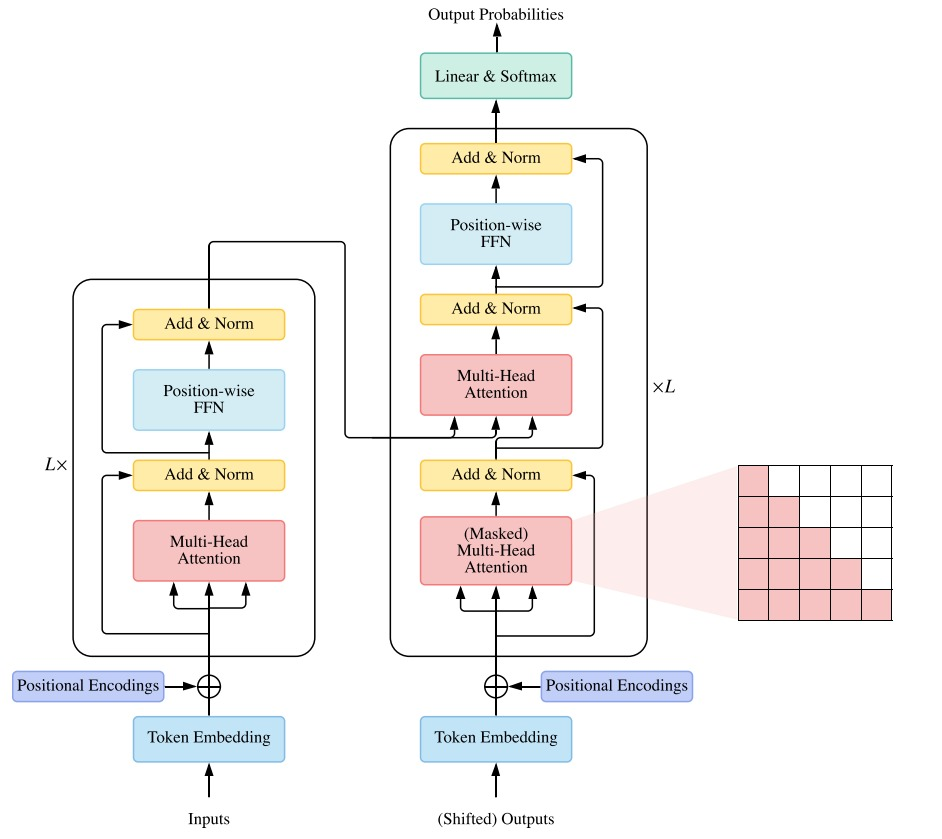
\includegraphics[width=12cm]{Cap2_LitReview/model_basics/Transformers/transformer_arch.png}
    \caption{Architecture of the vanilla Transformer model, with encoder and decoder components. \cite{lin2021surveytransformers}}
    \label{fig:Transformer-arch}
\end{figure}

The encoder is composed of a stack of L identical blocks. Each block is composed by two sub-layers: a multi-head attention and a feed-forward network. The multi-head attention sublayer is composed of H attention blocks, that use different projection matrices $\boldsymbol{W}_K$, $\boldsymbol{W}_V$ and $\boldsymbol{W}_Q$ to compute the key, value and query vectors, respectively. The output of each attention block is then concatenated and multiplied by a matrix $\boldsymbol{W}^O$, as shown in Equation \ref{eq:Transformer-MHA}:
\begin{equation}
    \text{MultiHead}(\boldsymbol{Q}, \boldsymbol{K}, \boldsymbol{V}) = \left(\text{head}_1;...;\text{head}_H\right) \cdot \boldsymbol{W}^O 
    \label{eq:Transformer-MHA}
\end{equation}
where $\text{head}_i = \text{Attention}(\boldsymbol{Q}\boldsymbol{W}_{i}^{Q}, \boldsymbol{K}\boldsymbol{W}_{i}^{K}, \boldsymbol{V}\boldsymbol{W}_{i}^{V})$ is the i-th attention head, and $\text{Attention}$ is the attention function defined in Section \ref{sec-attention}. 

A residual connection and layer normalization follow the multi-head attention, as shown in Equation \ref{eq:MHA-output}:
\begin{equation}
    \boldsymbol{H}' = \text{LayerNorm}(\text{MultiHead}(\boldsymbol{Q}, \boldsymbol{K}, \boldsymbol{V}) + \boldsymbol{X})
    \label{eq:MHA-output}
\end{equation}
where $\boldsymbol{X}$ is the input to the multi-head attention sublayer and $\text{LayerNorm}$ is the layer normalization function. The output $\boldsymbol{H}'$ is then processed by a position-wise feed-forward network with two fully connected layers: \ref{eq:Transformer-FFN}:
\begin{equation}
    \text{FFN}(\boldsymbol{H}') = \text{ReLU}(\boldsymbol{H}'\boldsymbol{W}_1 + \boldsymbol{b}_1)\boldsymbol{W}_2 + \boldsymbol{b}_2
    \label{eq:Transformer-FFN}
\end{equation}

The decoder has a similar architecture to the encoder. It has L stacked blocks, but each block is composed of three sub-layers: a masked multi-head attention layer, a multi-head attention layer, and a feed-forward network. The masked multi-head attention layer works similarly to the multi-head attention, but the self-attention is masked to prevent the model from attending to future tokens in the sequence, ensuring that the prediction for a given token only depends on the previous tokens \cite{lin2021surveytransformers}. Another difference is in the second multi-head attention layer, which uses the output of the encoder $\boldsymbol{Z}$ to project the key and value vectors of the attention.

Finally, one important point to highlight is the positional encoding layer. In vanilla transformers, the model does not have access to the order of the sequence. To deal with this, Vaswani et al. \cite{vaswani2023attentionneed} propose adding a positional encoding to the input. They do so using the sine and cosine functions:
\begin{equation}
    PE_{(pos,2i)} = \sin\left(\frac{pos}{10000^{2i/d_{model}}}\right)
\end{equation}
\begin{equation}
    PE_{(pos,2i+1)} = \cos\left(\frac{pos}{10000^{2i/d_{model}}}\right)
\end{equation}
where $i$ is the dimension, $pos$ is the token position and $d_{model}$ is the model dimension.


\section{Reconstruction-Based Models}

Reconstruction-based models are a class of machine learning models that are designed to learn the intrinsic correlations in data by trying to reconstruct the original input signal. Differently from forecasting-based approaches, which attempt to predict future values, reconstruction-based models focus on accurately recreating the current input. This approach makes them great for anomaly detection, often outperforming forecasting-based models because they have access to the current time series data, which helps them to be more stable to rapidly changing time series. However, this advantage comes with a trade-off because they introduce a delay in the detection of anomalies as they rely on reconstruction error analysis. \cite{Zamanzadeh_Darban_Webb_Pan_Aggarwal_Salehi_2024}. 

The main idea behind these networks is to train them to accurately reconstruct normal data, which is presumed to be the majority of the available data. This is usually done by minimizing a reconstruction loss, such as the Mean Squared Error (MSE), during the training phase. 

During the test phase, the model encounters anomalous data, which it has not been trained to reconstruct, causing the reconstruction error to increase greatly compared to the error of normal data, as the model fails to reconstruct abnormal patterns. This way, an anomaly can be identified by thresholding the reconstruction error. Inputs with low reconstruction error will be classified as normal, and inputs with reconstruction error greater than the threshold will be classified as anomalous.

There are a variety of reconstruction-based models. In Lachekhab et al. \cite{en17102340}, the authors proposed an autoencoder composed of multiple LSTM cells to identify anomalies in electrical motors vibrations. The model was trained using the MSE loss function to reconstruct normal vibration patterns, and anomalies were detected by applying a threshold to the reconstruction error.

In Xie, Xu and Jiang \cite{XIE2023120725}, the authors developed a model that combines convolutional layers, LSTM layers and a variational autoencoder to detect anomalies in multivariate time series. They computed correlation matrices between the variables to use as an input for the model and used a loss function that combines the MSE loss to the Kullback-Leibler divergence to train the model, achieving state-of-the-art results in three different datasets.

Another example is the model proposed in Tuli, Casale and Jennings \cite{tuli2022tranaddeeptransformernetworks} where authors utilized the transformer architecture to detect anomalies. The model works on two phases: in the first phase the model tries to reconstruct the input sequence, obtaining a reconstruction error. From this, the model computes the focus score that highlight areas with bigger reconstruction errors. In the second phase, the focus score is used by the attention mechanism to focus on areas where the reconstruction error was bigger, allowing the model to concentrate on these high-error regions and attempt a refined reconstruction. This approach allowed the authors to outperform state-of-the-art models on six different datasets.

\section{Railway Components}

The railway track consists of different interdependent components that are divided into two categories: the superstructure and the substructure. The former comprises the rails, fastenings, and sleepers, while the latter consists of the ballast, sub-ballast, and subgrade \cite{kaewunruen12008dynamic}, as shown in Figure \ref{fig:Track-Components}. These two structures are separated by the sleeper-ballast interface and are essential for ensuring a safe and cost-effective transportation system capable of guiding vehicles and transmitting loads to the subgrade \cite{attoh2017big}.

\begin{figure}[H]
    \centering
    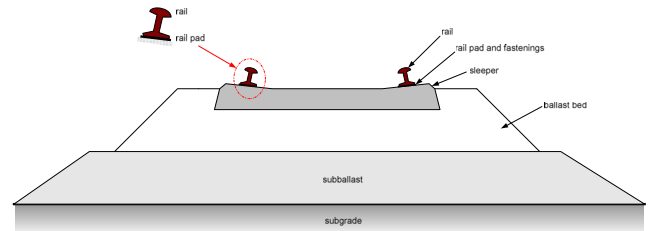
\includegraphics[width=12cm]{Cap2_LitReview/Track Components/track_components.png}
    \caption{Main railway track components, including superstructure and substructure. \cite{kaewunruen12008dynamic}}
    \label{fig:Track-Components}
\end{figure}

\section{Track Irregularities Standards} \label{sec-track-defects}

Railway track irregularities are deviations from the ideal track geometry that can affect the safety and comfort of train operations \cite{Sansinena26032025}. So, to ensure safe and efficient railway operations, a continuous assessment of track condition is necessary to support planning of maintenance actions. For this reason, different countries have established standards that quantify the characteristics of the track and their acceptable limits. In subsections \ref{sec-FRA-Standard} and \ref{sec-Brazil-Standard}, two of these standards will be presented: the Federal Railroad Administration (FRA) standard, used in the United States, and the Brazilian standard, used in Brazil.

\subsection{FRA Standard} \label{sec-FRA-Standard}

Railway track irregularities are normally modeled as being random and, for this reason, are typically described by a Power Spectral Density (PSD) function. Countries like USA, China, Britain and Germany adopted this approach to describe track irregularities \cite{PIRES2021107806,Berawi2013ImprovingRT}. The PSD function parameters were estimated from measured data and, therefore, represent the average irregularity observed in each respective railway network.

FRA classifies tracks into nine categories based on their condition, assigning a PSD function to each category. Categories 1 to 6 are designed for ordinary tracks, while categories 7 to 9 are intended for high-speed tracks. Due to equipment limitations, the FRA standard can only describe irregularities with wavelengths between 1.524 m to 304.8 m \cite{Berawi2013ImprovingRT}.

The PSD formulas are given by Equations \ref{eq:FRA-vertical}, \ref{eq:FRA-lateral} and \ref{eq:FRA-gauge}:

\begin{equation}
    S_{av}(\Omega) = \frac{k \cdot A_v \cdot \Omega_c^2}{\Omega^2 \cdot \left(\Omega^2 + \Omega_c^2\right)}
    \label{eq:FRA-vertical}
\end{equation}

\begin{equation}
    S_{al}(\lambda) = \frac{k \cdot A_a \cdot \Omega_c^2}{\Omega^2 \cdot \left(\Omega^2 + \Omega_c^2\right)}
    \label{eq:FRA-lateral}
\end{equation}

\begin{equation}
    S_{gauge/cl}(\lambda) = \frac{4 \cdot k \cdot A_v \cdot \Omega_c^2}{\left(\Omega^2 + \Omega_c^2\right) \cdot \left(\Omega^2 + \Omega_s^2\right)}
    \label{eq:FRA-gauge}
\end{equation}
where $S_{av}(\Omega)$ is the vertical alignment PSD, $S_{al}(\Omega)$ is the lateral alignment PSD, and $S_{gauge/cl}(\Omega)$ is the gauge or the superelevation PSD, all expressed in $[cm^2 / (rad/m)]$. The variable $\Omega$ is the spatial wavenumber, while $\Omega_c$ and $\Omega_s$ are the critical wavenumbers, all in $[rad/m]$. The variable $k$ is a constant, and $A_v$ and $A_a$ are the roughness coefficients related to the line grade, expressed in $[cm^2 \cdot rad /m]$. Table \ref{tab:FRA-PSD-parameters} summarizes the parameters for each track class.

\begin{table}[h!]
\centering
\resizebox{\textwidth}{!}{%
\begin{tabular}{c c c c c c c}
\hline
\multirow{2}{*}{Class} & \multicolumn{2}{c}{Max velocity (km/h)} & \multicolumn{4}{c}{Parameters} \\ \cline{2-7}
 & Freight & Passengers & $A_v$ (cm$^2$ rad/m) & $A_a$ (cm$^2$ rad/m) & $\Omega_c^2$ (rad/m) & $\Omega_s^2$ (rad/m) \\
\hline
1 & 16  & 24  & 1.2107 & 3.3634 & 0.6046 & 0.8245 \\
2 & 40  & 48  & 1.0181 & 1.2107 & 0.9308 & 0.8245 \\
3 & 64  & 97  & 0.6816 & 0.4128 & 0.8520 & 0.8245 \\
4 & 97  & 129 & 0.5376 & 0.3027 & 1.1312 & 0.8245 \\
5 & 129 & 145 & 0.2095 & 0.0762 & 0.8209 & 0.8245 \\
6 & 177 & 177 & 0.0339 & 0.0339 & 0.4380 & 0.8245 \\
\hline
\end{tabular}%
}
\caption{Summary of the parameters for each track class. \cite{PIRES2021107806}}
\label{tab:FRA-PSD-parameters}
\end{table}

One important point to highlight is that track condition in USA have very similar conditions to those in Brazil. For this reason, the FRA standard can be used to describe track irregularities in Brazil \cite{PIRES2021107806}.

\subsection{Brazilian Standard} \label{sec-Brazil-Standard}

The Brazilian Standard ABNT NBR 16387/2020 \cite{abnt:nbr16387:2020} specifies the geometrical limits for various railway track parameters, as presented in Table \ref{tab:track_geometry_limits}. It is important to note that these limits are related to the track irregularity profile but are not identical to it. To obtain the corresponding value for each geometry parameter, a specific function must be applied to the irregularity profile, converting it into a value that can be directly compared to the standard's limits. This procedure will later be used to label the track profiles, with irregularities exceeding the limits classified as defects.

\begin{table}[H]
\centering
\resizebox{\textwidth}{!}{%
\begin{tabular}{|p{5cm}|c|c|c|c|c|c|}
\hline
\textbf{Description of track geometry parameter} & \textbf{Gauge} & \textbf{(0--15) km/h} & \textbf{(16--40) km/h} & \textbf{(41--64) km/h} & \textbf{(65--95) km/h} & \textbf{(96--128) km/h} \\ \hline

\multicolumn{7}{|l|}{\textbf{Gauge}} \\ \hline
\textbf{Open gauge limit} (Static gauge) & Meter & 1035 mm & 1032 mm & 1032 mm & 1025 mm & 1013 mm \\ \hline
\textbf{Closed gauge limit} (Static gauge) & Meter & 987 mm & 987 mm & 987 mm & 987 mm & 987 mm \\ \hline
\textbf{Rapid gauge variation in 5 m} (Static gauge) & Meter & 34 mm & 31 mm & 23 mm & 18 mm & 13 mm \\ \hline

\multicolumn{7}{|l|}{\textbf{Crosslevel}} \\ \hline
\textbf{Crosslevel variation every 2 m} (Tangent) & Meter & 47 mm & 34 mm & 21 mm & 7 mm & 6 mm \\ \hline
\textbf{Crosslevel variation every 2 m} (Curve) & Meter & 18 mm & 14 mm & 11 mm & 5 mm & 3 mm \\ \hline
\textbf{Crosslevel variation every 10 m} & Meter & 53 mm & 37 mm & 33 mm & 31 mm & 30 mm \\ \hline

\multicolumn{7}{|l|}{\textbf{Alignment}} \\ \hline
\textbf{Curve misalignment in 10 m:} Maximum horizontal offset between adjacent points measured every 2.5 m at the mid-chord of 10 m & Meter & 31 mm & 24 mm & 18 mm & 13 mm & 8 mm \\ \hline
\textbf{Tangent alignment defect:} Maximum horizontal offset between adjacent points measured every 2.5 m at the mid-chord of 10 m & Meter & 31 mm & 24 mm & 18 mm & 13 mm & 8 mm \\ \hline

\multicolumn{7}{|l|}{\textbf{Curvature}} \\ \hline
\textbf{Maximum superelevation in curve} & Meter & 100 mm & 100 mm & 100 mm & 100 mm & 100 mm \\ \hline
\end{tabular}%
}
\caption{Limit values for the track geometry parameters. \cite{abnt:nbr16387:2020}}
\label{tab:track_geometry_limits}
\end{table}

\section{Assessing Railway Track Condition} \label{sec-assessing-railway-track}

Maintaining railway tracks in good condition is crucial to ensure safe and comfortable operations of trains \cite{Tsunashima-2019,GHIASI2025109516}. This maintenance is achieved through continuous monitoring of track conditions and the detection of irregularities. There are now two main methods to assess track quality: using track geometry cars (TGC) to directly measure the physical geometry of the track, and monitoring the dynamic response of the train using instrumented railway vehicles (IRV) equipped with onboard sensors capable of measuring the dynamics of the system \cite{PIRES2024107191}.

TGCs are equipped with sophisticated systems that directly measure the geometry of the track, that can be later compared to regulatory standards limits to identify parts of the track that need maintenance. However, this method has several drawbacks \cite{PIRES2024107191,GHIASI2025109516,Hironori_ONO202322-00239}:
\begin{itemize}
    \item \textbf{Operational disruption}: the operation of the railway track needs to be disrupted during the TGC inspection, which can halt operations for several hours depending on the length of the track being measured;
    \item \textbf{Operational high cost}: the sophisticated equipment and logistics make TGC operation costly, which limits their frequent use;
    \item \textbf{Low inspection frequency}: normally, the TGC measures the condition of the track monthly, due to its high cost, which is a problem if a fault appears between inspections.
\end{itemize}

To overcome the limitations in TGCs, an alternative approach was developed using IRVs equipped with sensors that measure the vehicle's dynamic response due to track excitations. The underlying principle behind IRVs is that the vehicle's vibrations are deeply correlated to track excitations, and an irregularity in the track will cause an anomalous dynamic response from the vehicle, which can be identified in the sensors' readings.

Using IRVs instead of the TGCs has several advantages, such as \cite{PIRES2024107191,GHIASI2025109516,Hironori_ONO202322-00239}:
\begin{itemize}
    \item \textbf{No disruptions}: the operation is not halted during the measurements, since data can be collected during normal train services, which reduces the costs with logistics;
    \item \textbf{Real time data collection}: data is collected in real time, which speeds up possible defect detections;
    \item \textbf{High frequency of inspections}: Since the measurements are taken directly from in-service trains, IRVs enable near-continuous monitoring of track conditions, greatly increasing the inspection frequency.
\end{itemize}

Despite that, it is important to highlight that data collection using IRVs also comes with some drawbacks, such as \cite{PIRES2024107191,GHIASI2025109516}:
\begin{itemize}
    \item High amount of data: the amount of data collected during IRV operation can be huge. This data needs to be carefully processed to obtain good quality data;
    \item Domain problem: different operations conditions, such as the wagon mass or velocity, can affect the dynamic response of the vehicle, so data collected from a one part of the track can be inherently different from another part;
    \item Difficult Correlation: since the measurements are done indirectly, they need to be correlated to the track condition, which can be a complex task that often needs the use of deep learning models;
    \item Data imbalance: since fault measurements are much more uncommon than normal measurements, the machine learning model needs to deal with class imbalance.
\end{itemize}

\section{Effect of the Velocity on Train Dynamics} \label{sec-vel-effect-measurement}

Train vibration measurements are strongly correlated to the velocity at which these measurements took place. As the wagon moves along the track, changes in velocity can alter the vibration responses measured by onboard sensors. Figure \ref{fig:vel_effect_ono} shows the difference in measurement found by \cite{Hironori_ONO202322-00239}. In Figure \ref{fig:vel_effect_ono-a}, the authors highlight two distinct velocity profiles labeled A and B, where the speed ratio between B and A is approximately 3. This difference in speed causes a significant change in the measured signal, as shown in Figure \ref{fig:vel_effect_ono-b}, where the velocity profile B resulted in higher acceleration measurements than A despite them traversing the same part of the track. At lower speeds, the dynamic response of the train to the track excitations tends to yield lower acceleration values, while, higher velocities tend to generate higher values of acceleration measured.

To address this velocity-induced distortion, the authors propose two different correction methods. The first method involves using the Mahalanobis distance \cite{de2000mahalanobis} to distinguish outliers from normal data. After that, the authors fitted a linear regression to normal data to predict the expected acceleration given the speed. The measurements are then normalized by dividing them by their predicted values.

In the second method, the authors employed a Gaussian process regression \cite{williams1995gaussian} to model the behavior of acceleration and speed, obtaining a regression that mapped the velocity to the expected acceleration. Similarly, they normalized the measurements by their respective predictions. 

Both methods proved to be effective in mitigating the velocity effect, which reduced the number of false positives in anomaly detection, as shown in Figure \ref{fig:vel_correction_ono}.

\begin{figure}[H]
    \centering
    \begin{subfigure}{0.45\textwidth}
        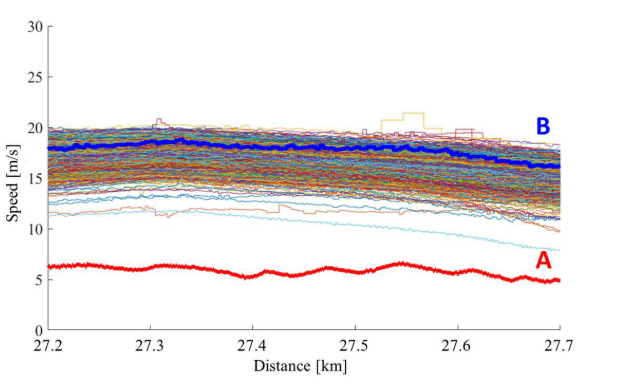
\includegraphics[width=8cm]{Cap2_LitReview/Vel_effect/vel_profiles.png}
        \caption{}
        \label{fig:vel_effect_ono-a}
    \end{subfigure}
    \hspace{0.3cm}
    \begin{subfigure}{0.45\textwidth}
        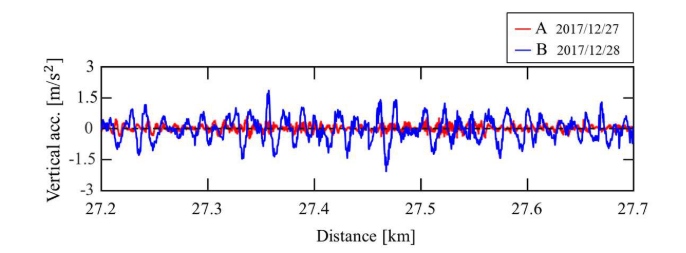
\includegraphics[width=8cm]{Cap2_LitReview/Vel_effect/accel_measurements.png}
        \caption{}
        \label{fig:vel_effect_ono-b}
    \end{subfigure}
    \caption{Example of how velocity differences affect acceleration measurements on the same track segment. $\boldsymbol{(a)}$ shows the two velocity profiles, A and B. $\boldsymbol{(b)}$ illustrates the corresponding acceleration measurements for each profile. Adapted from \cite{Hironori_ONO202322-00239}}
    \label{fig:vel_effect_ono}
\end{figure}

\begin{figure}[H]
    \centering
    \begin{subfigure}{0.45\textwidth}
        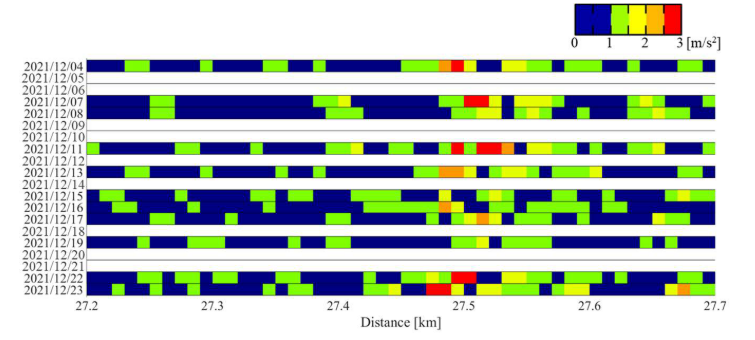
\includegraphics[width=8cm]{Cap2_LitReview/Vel_effect/before_correction.png}
        \caption{}
        \label{fig:vel_correction_ono-a}
    \end{subfigure}
    \hspace{0.3cm}
    \begin{subfigure}{0.45\textwidth}
        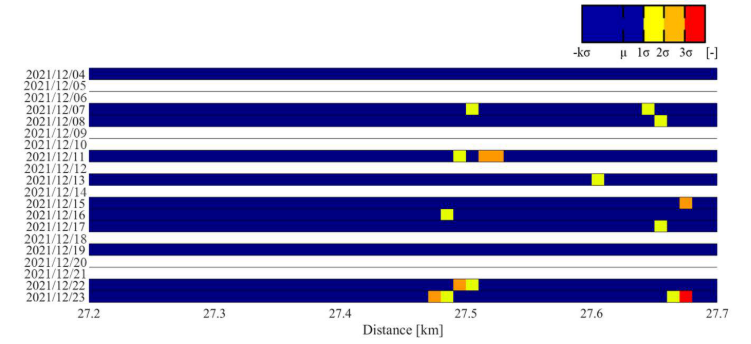
\includegraphics[width=8cm]{Cap2_LitReview/Vel_effect/after_correction.png}
        \caption{}
        \label{fig:vel_correction_ono-b}
    \end{subfigure}
    \caption{Reduction of false positives in anomaly detection after velocity correction. $\boldsymbol{(a)}$ shows the heatmap of the acceleration measurements before correction, while $\boldsymbol{(b)}$ shows the heatmap after correction. Adapted from \cite{Hironori_ONO202322-00239}}
    \label{fig:vel_correction_ono}
\end{figure}

Another example demonstrating the impact of the velocity on measured acceleration is presented in Balouchi, Bevan and Formston \cite{Balouchi02092021}. In this work, the authors utilized the VAMPIRE vehicle dynamics simulation software to model a vehicle operating in a measured track geometry at a variety of speeds. The simulated results were then compared to the actual car body vibration measurements recorded over the same section of the track. The results are shown in Figure \ref{fig:vel_effect_balouchi}, where the continuous colored lines are the simulation results, blue circles represent the maximum acceleration found in the simulation, and the dashed lines are the car body measurements. 

The authors fitted two models to the maximum simulated accelerations: a linear regression (green line) and an exponential model (purple curve), as shown in Figure \ref{fig:vel_effect_balouchi}. Based on the higher $R^2$ value, they selected the exponential model as the more suitable fit. They further argue that, at lower speeds, the acceleration response does not provide sufficient confidence to distinguish whether the track quality is good or poor. Therefore, a normalization approach, similar to that proposed by One et al. \cite{Hironori_ONO202322-00239}, is required.

\begin{figure}[H]
    \centering
    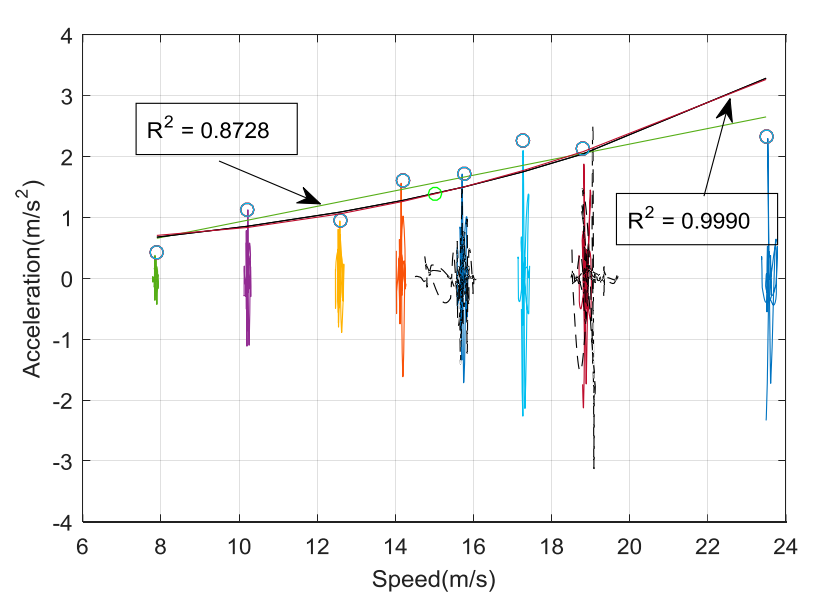
\includegraphics[width=12cm]{Cap2_LitReview/Vel_effect/results_bia.png}
    \caption{Effect of train velocity on measured acceleration compared with simulation results and the linear and exponential model fitted to the maximum acceleration values with their corresponding $R^2$ values \cite{Balouchi02092021}.}
    \label{fig:vel_effect_balouchi}
\end{figure}

In the two papers above, the authors show the importance of correcting the acceleration measurements acquired at different velocities, as variations in speed alter the dynamic response of the train. However, their correction only considers the effect of the velocity and not the effect of the mass, as these studies were performed in a passenger car. In this type of vehicle, the mass doesn't vary significantly, as it carries passengers which are way lighter compared to the raw materials transported by heavy haul wagons. Section \ref{sec-mass-effect-measurement} will show that the mass of the train might also affect the dynamics of the system.

\section{Effect of Mass on Train Dynamics} \label{sec-mass-effect-measurement}

When analyzing the data collected by an IRV in a Brazilian railway, described in detail in Pires et al. \cite{PIRES2024107191}, it was noticed that the mass of the wagon influences the relationship between acceleration growth and velocity. This phenomenon is illustrated in Figure \ref{fig:mass_effect}, which shows the 99th percentile of the absolute maximum vertical acceleration as a function of the velocity class. Each velocity class corresponds to data points that have a velocity between an 1 m/s interval. For example, the velocity class $7 < v < 8$ corresponds to all data points whose velocity is between 7 m/s and 8 m/s.

In the Figure, data points are colored according to the wagon mass class. The unloaded class corresponds to an empty wagon, i.e, that is not transporting any material, the loaded class corresponds to a wagon fully loaded with iron ore, and the $1/4$ to $3/4$ classes correspond to wagons that were either partially loaded or carrying lighter materials such as coal. One point to highlight, is that it was used the 99th percentile instead of the maximum value because the dataset consists of real-world measurements, which are prone to noise and outliers.

As shown in the Figure, different wagon masses produce distinct acceleration growth behavior: the unloaded wagon exhibits the lowest acceleration growth, the $1/4$ loaded wagon shows a slightly higher growth, and the $2/4$, $3/4$, and fully loaded wagons display similar growth patterns.

These observations highlight the need to further investigate the correlation between wagon mass and velocity behavior for freight operations.

\begin{figure}[H]
    \centering
    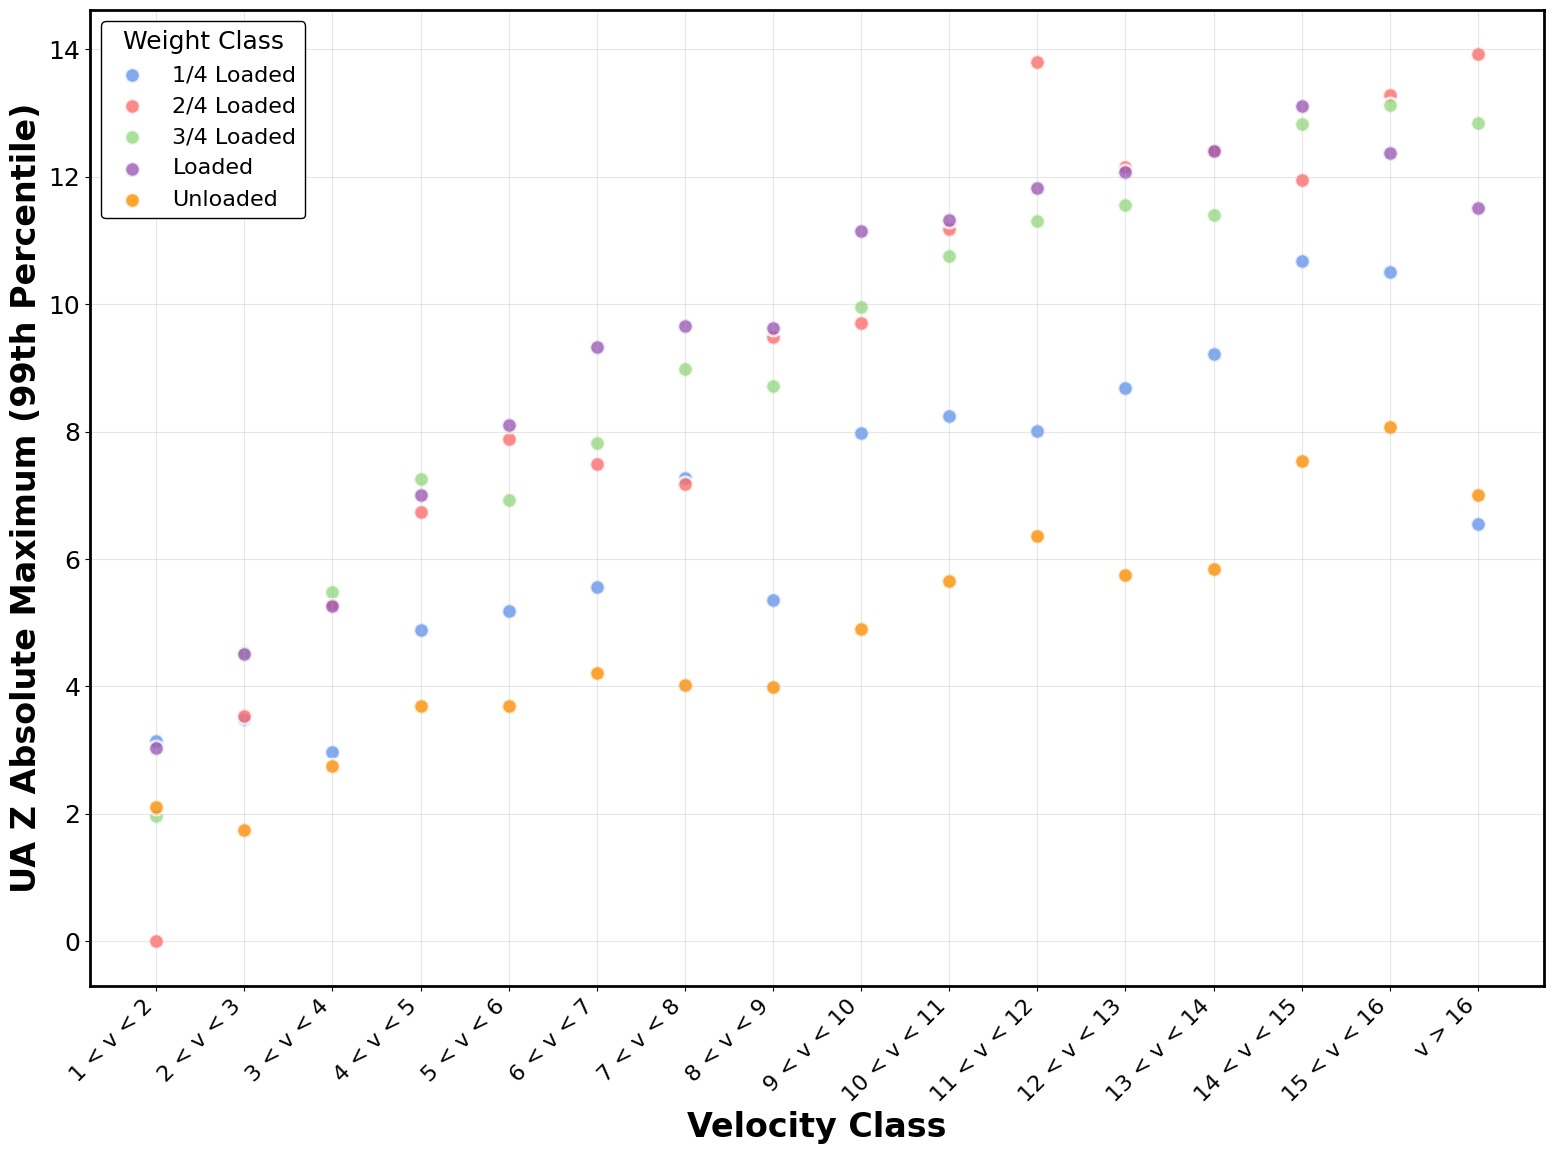
\includegraphics[width=12cm]{Cap2_LitReview/Mass_effect/Mass_effect.jpg}
    \caption{Effect of wagon mass on the relationship between acceleration and velocity for freight trains. The data points represent the 99th percentile of the absolute maximum vertical acceleration for each velocity class, colored by wagon mass class.}
    \label{fig:mass_effect}
\end{figure}

\section{Assessing Track Irregularities from Acceleration Data} \label{sec-track-quality-accel}

In Sansinena, Rodríguez-Arana and Arrizabalaga \cite{Sansinena26032025} authors presented a review of research papers that proposed methods for estimating track irregularities using acceleration data. They divided the methods into three main categories:
\begin{itemize}
    \item Model-driven methods;
    \item Data-driven methods;
    \item Hybrid methods.
\end{itemize}

In model-driven methods, a mathematical representation of the dynamic system is developed and validated on real data. Once the model accurately represents the system dynamics, the problem is inverted to estimate track irregularities from the measured acceleration data. The main advantage in model-driven methods is that they don't require a large amount of data to be designed, as they're based on expert knowledge. 

For instance, in De Rosa, Alfi and Bruni \cite{DEROSA2019606} the authors used a 3D multibody model that was previously validated to measure the yaw and roll motions of the vehicle. Based on simulation data, they applied three reconstruction techniques, the Kalman filter, the Unknown Input Observer (UIO) and the Frequency Response Function (FRF), to reconstruct the lateral irregularities and the cross alignment. The performance of these methods were compared using two evaluation metrics $J_y$ and $J_\rho$, defined by Equations \ref{eq:DeRosa-Jy} and \ref{eq:DeRosa-Jrho}: 
\begin{equation}
    J_y = \frac{\text{rms}(y_{est} - y)}{\text{rms}(y)}
    \label{eq:DeRosa-Jy}
\end{equation} 
\begin{equation}
    J_\rho = \frac{\text{rms}(\rho_{est} - \rho)}{\text{rms}(\rho)}
    \label{eq:DeRosa-Jrho}
\end{equation}
where $y_{est}$ and $\rho_{est}$ are the estimated lateral and cross alignment irregularities, $y$ and $\rho$ are the original values and $\text{rms}$ is the root mean square function. The results for these two metrics are shown in Table \ref{tab:DeRosa_Results}, where values closer to 0 indicate a better performance and FD corresponds to the FRF function. 

\begin{table}[H]
\centering
\begin{tabular}{lccc}
    \hline
    & FD & UIO & KF \\
    \hline
    $\mathbf{J_y}$ & 0.325 & 0.291 & 0.363 \\
    $\mathbf{J_p}$ & 0.122 & 0.549 & 0.124 \\
    \hline
\end{tabular}
\caption{Comparison of the accuracy indices.}
\label{tab:DeRosa_Results}
\end{table}

From these results, the authors decided to use the FRF method on real measured data, which included lateral and vertical accelerations recorded at the axle-boxes, bogies, and car body. However, they did not report any quantitative metrics for the reconstruction of real irregularities, presenting only the results shown in Figure \ref{fig:DeRosa_Results}. The authors argue that although some similarity between the reconstructed and the original irregularities can be seen, the method did not produce visually satisfactory results. They justify that this deviation is caused by non-linear effects they didn't consider, but these deviations can occur because of the lack of robustness of the method to real-world noise in data, which is a common problem when dealing with simpler reconstruction methods.

\begin{figure}[H]
    \centering
    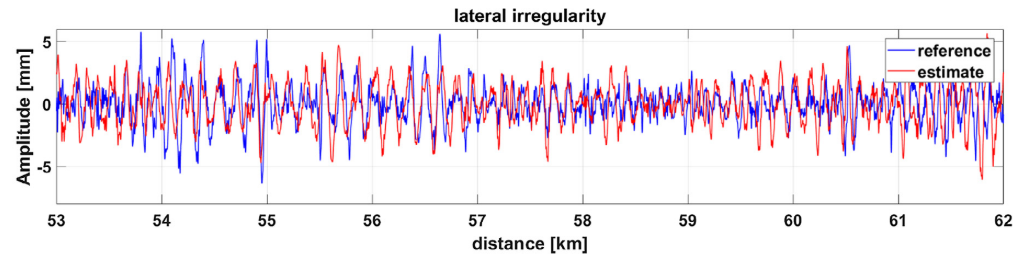
\includegraphics[width=12cm]{Cap2_LitReview/Track_Quality_Accel/DeRosa_Result_Real.png}
    \caption{Reconstruction of lateral irregularities using the Frequency Response Function method \cite{DEROSA2019606}.}
    \label{fig:DeRosa_Results}
\end{figure}

Data-driven methods, on the other hand, do not consider a mathematical model of the system, relying only on data processing to reconstruct or identify the irregularities. These methods typically utilize traditional machine learning algorithms or, more recently, deep learning architectures. Such approaches are generally more robust when dealing with real-world data, as they can learn from noisy and complex signals. This robustness, however, comes with a price, as they need a larger amount of data to be trained, especially in the case of deep learning \cite{Sansinena26032025}. 

In Tsunashima and Yagura \cite{vibration7040049} the authors propose a method of estimating railway track irregularities from car body vibration data. They first created a multibody simulation in SIMPACK. After that, they generated 12 different track irregularities, ranging from a good condition to a degraded condition, using FRA PSD formula and converted the generated profiles into 10 meters long track irregularity sections using the 10 m-chord versine method. This transformation is shown in Figure \ref{fig:Tsunashina_data_process}.

Using these irregularity profiles, they ran simulations over a 1000 meters track at speeds in the range of 40 to 80 km/h, varying the velocity in a 10 km/h interval. For each combination of track profile and speed, they collected the vertical and lateral acceleration as well as the roll rate of the carbody. Similarly to the irregularity profiles, a downsample was also applied to the data taking the maximum vibration measured in the 10 meters section, as shown in Figure \ref{fig:Tsunashina_data_process}. From this process, they obtained a dataset that correlates the maximum vibration of the carbody to the track irregularities for varying speeds and then applied a Gaussian Process Regressor (GPR) that was able to predict the irregularity from the vibration for a certain vehicle speed, as illustrated in Figure \ref{fig:Tsunashina_GPR}. 


\begin{figure}[H]
    \centering
    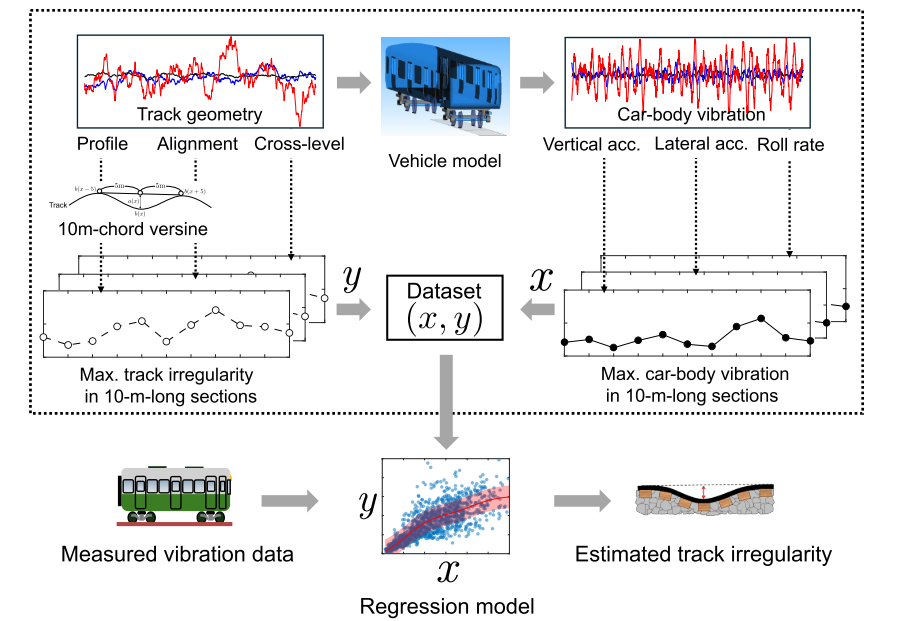
\includegraphics[width=12cm]{Cap2_LitReview/Track_Quality_Accel/Tsunashina (2024)/data-process.png}
    \caption{Data processing pipeline for the creation of the simulated dataset \cite{vibration7040049}.}
    \label{fig:Tsunashina_data_process}
\end{figure}

\begin{figure}[H]
    \centering
    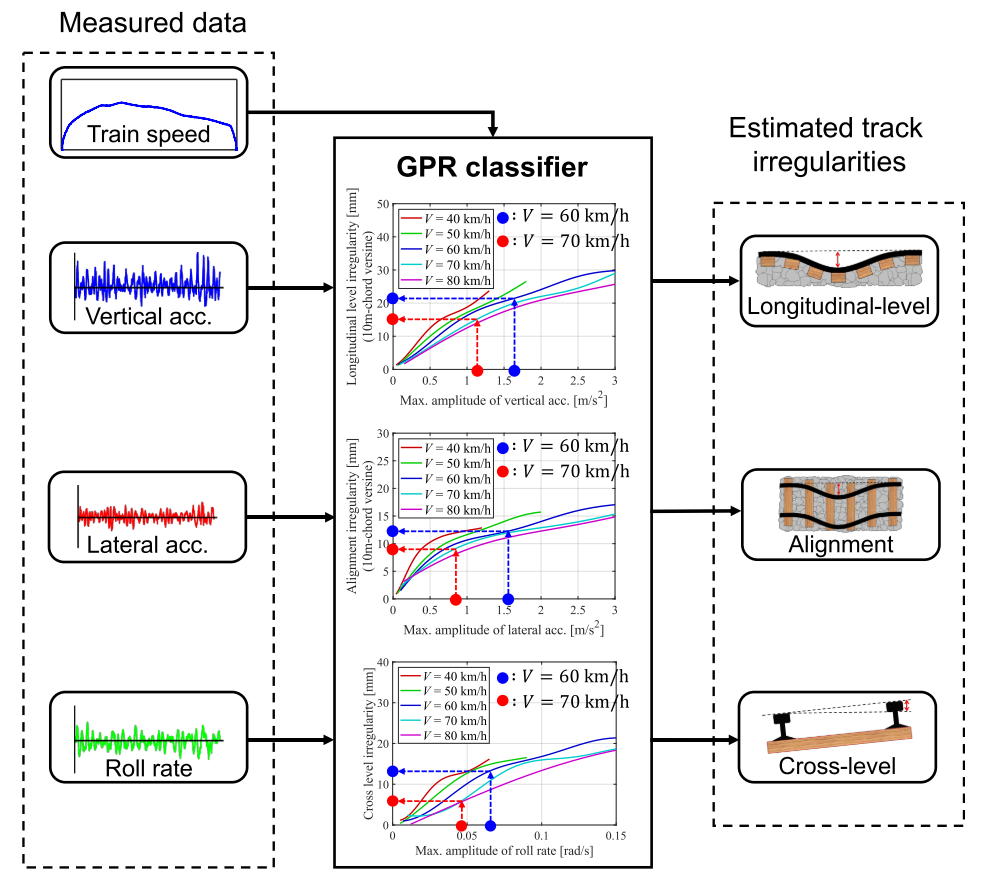
\includegraphics[width=12cm]{Cap2_LitReview/Track_Quality_Accel/Tsunashina (2024)/gpr.png}
    \caption{Track irregularity prediction using Gaussian Process Regression for different vehicle speeds \cite{vibration7040049}.}
    \label{fig:Tsunashina_GPR}
\end{figure}

The authors then validated their model using real data collected with an onboard sensing device equipped with a triaxial accelerometer to measure carbody acceleration, a rate gyro to capture the carbody roll rate, and a GNSS receiver to determine vehicle position. To ensure consistency, they applied the same downsample procedure to the real data and averaged the speed in the 10 m section to be used as an input for the regression model. The regression result for one part of the track is shown in Figure \ref{fig:Tsunashina_Results} and is presented with a 1$\sigma$ confidence interval. However, they didn't provide any quantitative metrics.

Tsunashima and Yagura argue that for the majority of the sections, the GPR predicts the correct value within the 1$\sigma$ confidence interval. However, for some of the sections, the predicted value significantly deviated from the actual measurement. They argue that there is a factor other than the track irregularity that influences the dynamics of the system and superimposes on the carbody's vibration. This difference might also occur because of the low complexity model used that might not have been able to learn the correlations between the variables very well. 

\begin{figure}[H]
    \centering
    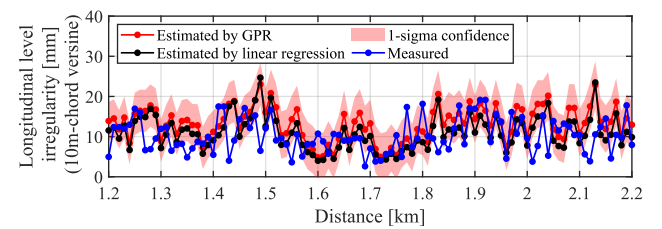
\includegraphics[width=12cm]{Cap2_LitReview/Track_Quality_Accel/Tsunashina (2024)/Results.png}
    \caption{Regression results comparing predicted and actual track irregularities from real measurement data. \cite{vibration7040049}}
    \label{fig:Tsunashina_Results}
\end{figure}

To address this model issue, Hao et al. \cite{Hao02012023} proposes a deep learning approach to reconstruct the track irregularity from vertical and lateral carbody acceleration measurements. The authors used a dataset composed of acceleration measurements collected in three high-speed Chinese railway lines. In the dataset, they also had access to the measured geometry of the track. Since they aimed to reconstruct irregularities with wavelengths between 3 m and 120 m, they applied a band-pass filter to remove components with wavelengths outside this range. They also decided to scale the data using a min-max scaler, although the authors are not clear if they do that to the entire dataset or if they apply it to each time window individually. Finally, since their data is measured with velocities between 40 and 310 km/h, they decided to give the vehicle speed as an input for the model.

They proposed a model that combines an attention mechanism with a 1D CNN layer and a GRU layer, allowing it to capture both spatial and temporal dependencies in the data. The model architecture is shown in Figure \ref{fig:Hao_model}. It receives vertical and lateral carbody acceleration, along with velocity, as inputs. The output was the vertical profile, that have wavelengths between 3 and 120 m, and the long-wave vertical profile, with wavelengths between 42 and 120 m. They trained and tested the proposed model using two different lines: the NHHSR and the BGHSR, and compared it to two simpler versions of the model. The results of the three models in the two lines are presented in Table \ref{tab:HAO_evaluation_indices}, where the best results are highlighted in bold. The evaluation metrics used were the Mean Absolute Error (MAE), Root Mean Square Error (RMSE), Theil Inequality Coefficient (TIC) and Pearson Correlation Coefficient (PCC), defined by:
\begin{equation}
MAE = \frac{1}{M} \sum_{k=1}^{M} \left| y_k - \hat{y}_k \right|.
\end{equation}
\begin{equation}
RMSE = \sqrt{ \frac{1}{M} \sum_{k=1}^{M} \left( y_k - \hat{y}_k \right)^2 }.
\end{equation}
\begin{equation}
TIC = \frac{ \sqrt{ \frac{1}{M} \sum_{k=1}^{M} \left( y_k - \hat{y}_k \right)^2 } }
{ \sqrt{ \frac{1}{M} \sum_{k=1}^{M} y_k^2 } + \sqrt{ \frac{1}{M} \sum_{k=1}^{M} \hat{y}_k^2 } }.
\end{equation}
\begin{equation}
PCC = \frac{ \sum_{k=1}^{M} \left( \hat{y}_k - \bar{\hat{y}} \right) \left( y_k - \bar{y} \right) }
{ \sqrt{ \sum_{k=1}^{M} \left( \hat{y}_k - \bar{\hat{y}} \right)^2 } 
\cdot \sqrt{ \sum_{k=1}^{M} \left( y_k - \bar{y} \right)^2 } },
\quad \left( \bar{y} = \frac{1}{M} \sum_{k=1}^{M} y_k, \;
\bar{\hat{y}} = \frac{1}{M} \sum_{k=1}^{M} \hat{y}_k \right).
\end{equation}
where $y$ is the actual value, $\hat{y}$ is the predicted value, $M$ is the number of samples, and $\bar{y}$ and $\bar{\hat{y}}$ are the mean values of $y$ and $\hat{y}$, respectively.

\begin{figure}[H]
    \centering
    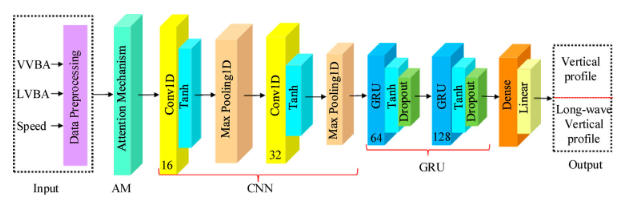
\includegraphics[width=12cm]{Cap2_LitReview/Track_Quality_Accel/Hao (2023)/Model_arch.png}
    \caption{Model architecture utilized to reconstruct the track irregularity \cite{Hao02012023}.}
    \label{fig:Hao_model}
\end{figure}

\begin{table}[H]
\centering
\begin{tabular}{llllcccc}
    \hline
    \textbf{HSR line} & \textbf{Model} & \textbf{Output} & \textbf{MAE} & \textbf{RMSE} & \textbf{TIC} & \textbf{PCC} \\ \hline
    \multirow{6}{*}{NHHSR} 
    & GRU & Long-wave vertical profile & 0.4995 & 0.6456 & 0.3801 & 0.7292 \\
    &     & Vertical profile           & 0.2720 & 0.3558 & 0.3834 & 0.7254 \\
    & CNN--GRU & Long-wave vertical profile & 0.4951 & 0.6393 & 0.3728 & 0.7392 \\
    &     & Vertical profile           & 0.2688 & 0.3521 & 0.3877 & 0.7293 \\
 & \textbf{AM--CNN--GRU} & Long-wave vertical profile & \textbf{0.4808} & \textbf{0.6205} & \textbf{0.3653} & \textbf{0.7513} \\
 &     & Vertical profile           & \textbf{0.2652} & \textbf{0.3459} & \textbf{0.3710} & \textbf{0.7425} \\ \hline
\multirow{6}{*}{BGHSR} 
& GRU & Long-wave vertical profile & 0.5048 & 0.6425 & 0.3303 & 0.7879 \\
 &     & Vertical profile           & 0.2934 & 0.3762 & 0.3442 & 0.7816 \\
 & CNN--GRU & Long-wave vertical profile & 0.5020 & 0.6360 & 0.3242 & 0.7932 \\
 &     & Vertical profile           & 0.2905 & 0.3717 & 0.3308 & 0.7919 \\
 & \textbf{AM--CNN--GRU} & Long-wave vertical profile & \textbf{0.5001} & \textbf{0.6355} & \textbf{0.3244} & \textbf{0.7935} \\
 &     & Vertical profile           & \textbf{0.2867} & \textbf{0.3668} & \textbf{0.3236} & \textbf{0.7975} \\ \hline
\end{tabular}
\caption{Evaluation metrics for different models and different lines \cite{Hao02012023}.}
\label{tab:HAO_evaluation_indices}
\end{table}

Figure \ref{fig:Hao_Results}

\begin{figure}[H]
    \centering
    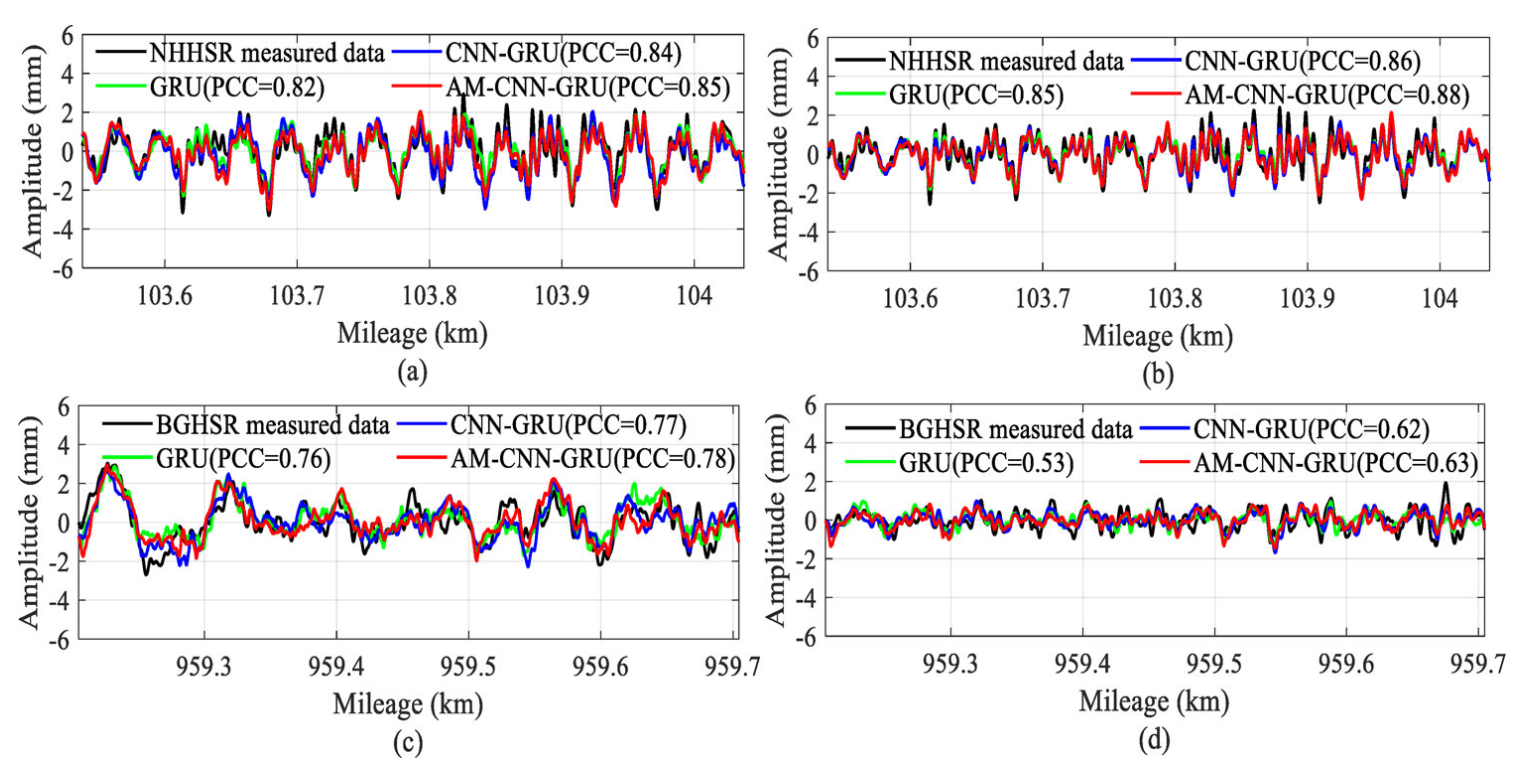
\includegraphics[width=12cm]{Cap2_LitReview/Track_Quality_Accel/Hao (2023)/Hao_results.png}
    \caption{Reconstruction results comparing the proposed model (red) with two simpler models (blue and green) and the original measurement (black). \cite{Hao02012023}}
    \label{fig:Hao_Results}
\end{figure}

The results show that the proposed approach achieved reconstructions much closer to the real measurements than the model-driven approach and a Gaussian Process Regression model, demonstrating its robustness in handling real-world noisy data. However, the model uses vehicle speed as an input, which may not be optimal. In this thesis, it is proposed instead to use corrected acceleration values.

Finally, hybrid methods combine the approaches of model-driven and data-driven methods, but the contents of these works are outside the scope of this thesis.

\section{Thresholding Acceleration Data} \label{sec-thresholding-acceleration}

In Rosa et al. \cite{DeRosa2021}, the authors try to develop a threshold to detect not safe railway track irregularities. In the paper, the authors propose a machine learning-based classification model that divides the data into two classes based on the standard deviation of the lateral and roll bogie frame accelerations. Class 1 corresponds to normal conditions, i.e., track irregularities below a defined threshold that do not require maintenance, while Class 2 corresponds to sections with irregularities exceeding that threshold, thus requiring maintenance intervention. 

The authors use a dataset composed of real measurements collected onboard the high-speed TGC, operating at 300 km/h, that was also equipped with accelerometers located on the carbody, the bogie frames and the wheelsets, and a set of simulated data generated using a validated multibody dynamics model. From real data, the athor applies a pass-band filter in the range of 3 to 27 Hz and then computed the standard deviation of the signals over 100-meter-long track length. The simulation data was obtained considering a straight track, with a vehicle with speed of 300 km/h and for three different cases of track irregularities: considering only the lateral irregularity, considering only the cross level irregularity, and considering both at the same time. The authors didn't consider vertical irregularities in their simulation. For each case, they ran the simulation 10 times. The standard deviation was computed similarly to the real data. Figure \ref{fig:DeRosa-dataset} shows the whole dataset, where the red lines shown the standard defined limits for the standard deviation.

Using this dataset, the authors then fitted the data three classifiers: a decision tree, a linear Support vector Machine (SVM) and a Gaussian SVM. Results are shown in Figure \ref{fig:DeRosa-2021-Results}. The authors, then, discuss the performance of each classifier, but, more importantly for this work, they show the possibility of defining a threshold in the standard deviation of acceleration data to classify the track condition. In this thesis, it will be tested if this threshold method can also be used in direct acceleration data instead of the standard deviation.

\begin{figure}[H]
    \centering
    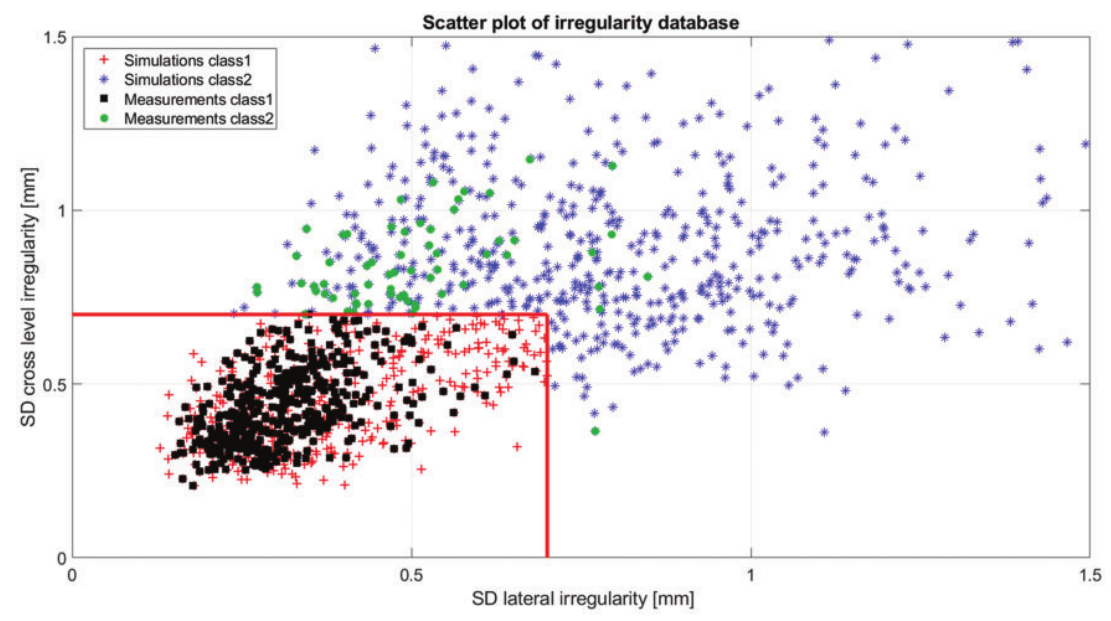
\includegraphics[width=12cm]{Cap2_LitReview/Track_Quality_Accel/DeRosa (2021)/dataset.png}
    \caption{Dataset distribution of standard deviation of the irregularities with defined safety thresholds. \cite{DeRosa2021}}
    \label{fig:DeRosa-dataset}
\end{figure}

\begin{figure}[H]
    \centering
    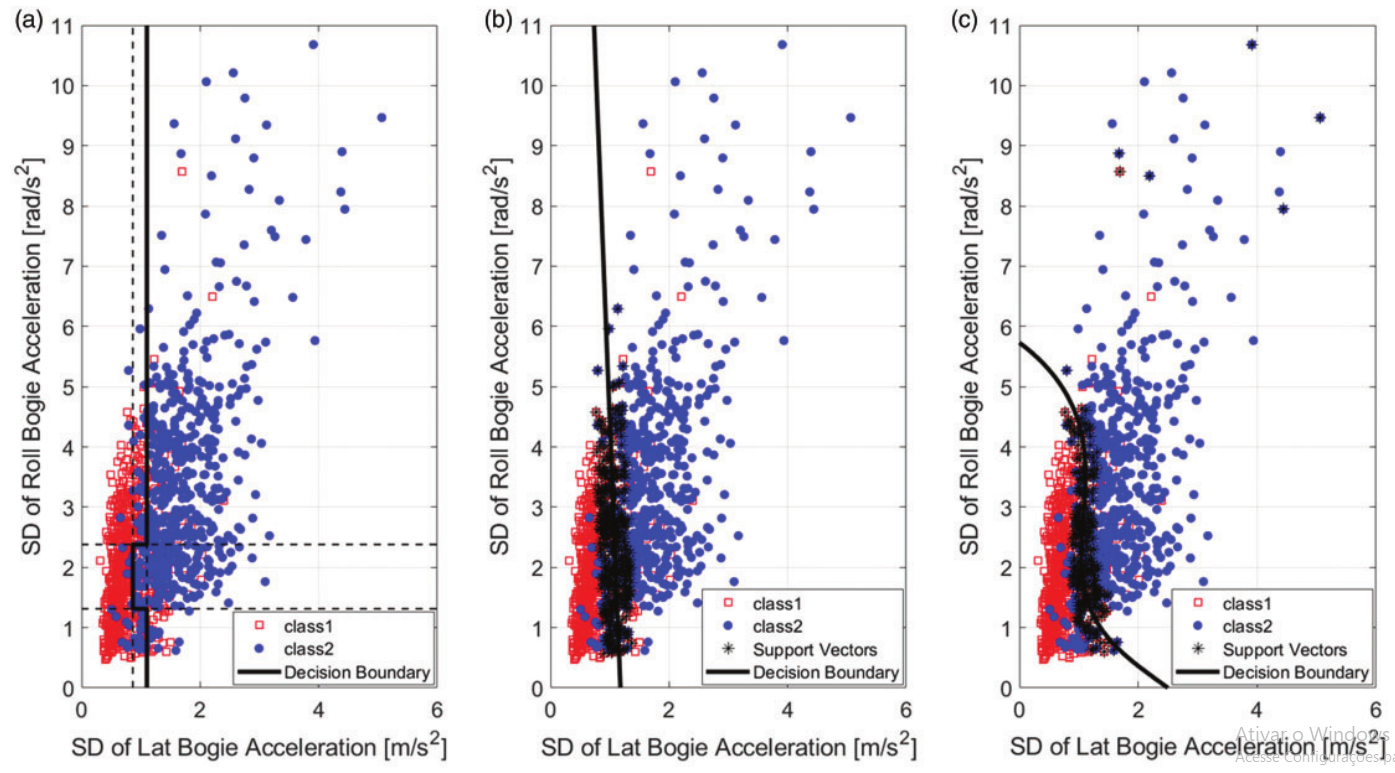
\includegraphics[width=12cm]{Cap2_LitReview/Track_Quality_Accel/DeRosa (2021)/Results.png}
    \caption{Classification results of the three classifiers on the test set. $\boldsymbol{(a)}$ the decision boundary for the decision tree. $\boldsymbol{(b)}$ the decision boundary for the linear SVM. $\boldsymbol{(c)}$ the decision boundary for the Gaussian SVM. \cite{DeRosa2021}}
    \label{fig:DeRosa-2021-Results}
\end{figure}

% \begin{table}[ht]
% \centering
% \begin{tabular}{l c c c c c}
% \hline
%  & Accuracy (\%) & Precision (\%) & Recall (\%) & $F_1$ score (\%) & Kappa \\
% \hline
% Decision tree & 87.6 & 49.6 & 92.1 & 64.4 & 0.58 \\
% Linear SVM & 92.9 & 70.3 & 71.4 & 70.9 & 0.67 \\
% Gaussian SVM & 92.9 & 68.1 & 77.8 & 72.6 & 0.69 \\
% \hline
% \end{tabular}
% \vspace{0.5em}
% \small SVM: support vector machine.
% \caption{Summary of classifier performances in the testing phase.}
% \label{Table:DeRosa-2021-Results}
% \end{table}


% \begin{figure}[H]
%     \centering
%     \begin{subfigure}{0.8\textwidth}
%         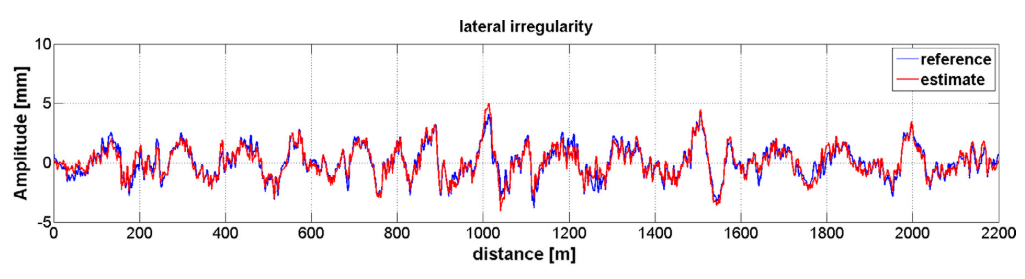
\includegraphics[width=8cm]{Cap2_LitReview/Track_Quality_Accel/DeRosa_Results_Freq.png}
%         \caption{Adapted from \cite{DEROSA2019606}}
%         \label{fig:deRosa_a}
%     \end{subfigure}
%     \\
%     \begin{subfigure}{0.8\textwidth}
%         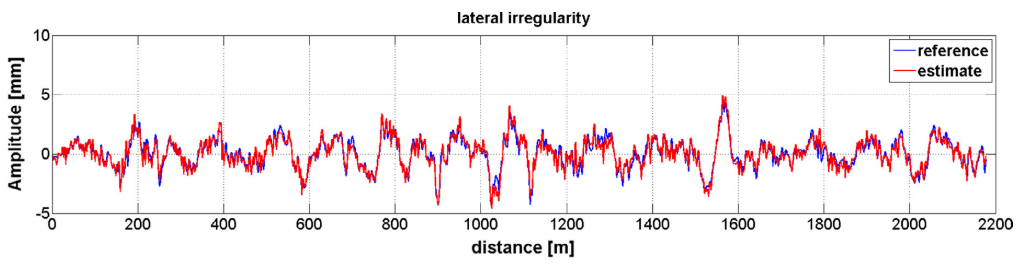
\includegraphics[width=8cm]{Cap2_LitReview/Track_Quality_Accel/DeRosa_Results_UIO.png}
%         \caption{Adapted from \cite{DEROSA2019606}}
%         \label{fig:deRosa_b}
%     \end{subfigure}
%     \\
%     \begin{subfigure}{0.8\textwidth}
%         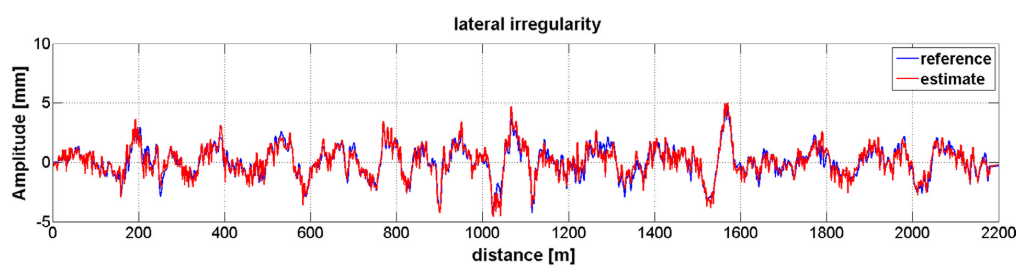
\includegraphics[width=8cm]{Cap2_LitReview/Track_Quality_Accel/DeRosa_Results_Kalman.png}
%         \caption{Adapted from \cite{DEROSA2019606}}
%         \label{fig:deRosa_c}
%     \end{subfigure}
%     \caption{Caption}
%     \label{fig:DeRosa_Results}
% \end{figure}

% \begin{table}[H]
% \centering
% \begin{tabular}{l c c c}
% \hline
%  & FD & UIO & KF \\
% \hline
% \textbf{No Noise} & & & \\
% \quad $\mathbf{J_y}$ & 0.325 & 0.291 & 0.363 \\
% \quad $\mathbf{J_p}$ & 0.122 & 0.549 & 0.124 \\
% \textbf{With Noise} & & & \\
% \quad $\mathbf{J_y}$ & 0.326 & 0.828 & 0.425 \\
% \quad $\mathbf{J_p}$ & 0.162 & 2.781 & 0.194 \\
% \hline
% \end{tabular}
% \caption{\cite{DEROSA2019606}}
% \label{table:DeRosa}
% \end{table}


%\section{Identifying Track Defects Using IRVs} \label{sec-IRV-track-defect-identification}

\chapter{Methodology} \label{sec-methodology}

This chapter describes the methodology used to develop a machine learning model that is capable of reconstructing the track irregularities from acceleration data. It is organized as follows: Section \ref{sec-defining-problem} defines the problem to be solved, Section \ref{sec-vel-mass-correction} describes the simulation parameters for the velocity and mass correction, Section \ref{sec-ml-model} describes the machine learning model that will be used to reconstruct the track irregularities, and Section \ref{sec-flowchart} presents a flowchart of the step by step methodology.

\section{Defining the Problem} \label{sec-defining-problem}

In this thesis, the main objective is to develop a machine learning model that can reconstruct track irregularities from acceleration data. The reconstructed profiles can be then compared to the standard limits to support maintenance planning, or, in the case of an off limits irregularity, a defect can be identified and repaired before it causes a serious issue.

To acquire data, a multibody simulation will be created in the software SIMPACK. First, the simulation model will be validated using real data from a section of track geometry measured by the TCG and the corresponding acceleration measurements collected by the IRV. The simulated wagon will replicate the IRV sensor configuration, described in detail in \cite{PIRES2024107191}, measuring the vertical acceleration on the side frames, the displacement of the secondary suspension and the triaxial carbody acceleration. Once the simulation is validated, a dataset will be generated containing the simulated sensor data for different track irregularities, velocities and for different wagon masses. This search space will be explained in more details in Section \ref{sec-vel-effect-measurement}.

With this dataset, a study will be conducted to analyze the effect of the wagon mass and velocity on the acceleration measurements. The goal is to understand how these parameters affect the data and develop a correction method, using similar approaches described in Sections \ref{sec-vel-effect-measurement} and \ref{sec-mass-effect-measurement}, to correct the acceleration data.

The corrected acceleration data will then be used to train a machine learning model for reconstructing track irregularities. Model performance will be evaluated using real-world data. Finally, a threshold will be defined on the reconstructed profiles to determine when maintenance is required, enabling condition-based planning based solely on acceleration measurements.

\section{Velocity and Mass Correction} \label{sec-vel-mass-correction}

As stated in Section \ref{sec-defining-problem} a SIMPACK simulation will run across a search space composed of different velocities, wagon masses and track irregularities. Table \ref{table:search_space} summarizes the parameter ranges. Each simulation will test one combination until all possibilities have been explored.

\begin{table}[H]
\centering
\begin{tabular}{l l}
\hline
\textbf{Parameter} & \textbf{Values} \\
\hline
Velocity (km/h) & 5, 10, 15, 20, 25, 30, 35, 40, 45, 50, 55, 60, 65 \\
Wagon mass (tons) & 0, 51, 102 \\
Track irregularity & No irregularity, FRA 6, FRA 5, FRA 4, Real Irregularity \\
\hline
\end{tabular}
\caption{Search space for the SIMPACK simulation.}
\label{table:search_space}
\end{table}

The velocity range was defined to cover the typical train velocity operation in the railway. Wagon masses corresponds to the unloaded wagon class, the half loaded wagon and the fully loaded wagon class. The track irregularities were defined to cover a good track condition (FRA 6), a regular condition track (FRA 5) and a bad condition track (FRA 4). The real irregularity corresponds to a measured track geometry that contains some defects, such as a switch and some misalignments. The no irregularity serves as a baseline case to the study.

From this generated data, an approach similar to \cite{Balouchi02092021} will be used to correct the measurements. In this method, a linear or quadratic regression model will be fitted to the absolute maximum acceleration data across different velocities and different wagon masses. The goal is to develop a correction method that is independent from the track irregularity. The final regression model will be evaluated on real world data.

\section{Machine Learning Model} \label{sec-ml-model}

The machine learning model to be used in this thesis needs to satisfy a set of requirements. These requirements are:
\begin{itemize}
    \item The model can not depend on labels, i.e., it needs to be an unsupervised model;
    \item The model should consider input data as being sequential, i.e., it needs to take into consideration temporal correlations;
    \item The model needs to be able to handle noisy data;
    \item The model should be able to be trained on simulated data and perform well on real world data without the need of retraining.
\end{itemize}

Based on these requirements, the chosen approach is to use a deep learning model that utilizes the methods described in Section \ref{sec-model-basics}, as it is the most robust approach for handling complex data. This outputs of this model will be then compared to the geometric limits in the Brazilian standard to develop a threshold for maintenance planning based on acceleration data.

\section{Flowchart} \label{sec-flowchart}

Figure \ref{fig:flowchart} presents the flowchart of the proposed methodology. The Figure illustrates the step-by-step process, starting from the creation and validation of the SIMPACK simulation, through the generation of the dataset with different velocities, wagon masses and track irregularities, to the correction of the acceleration data and the training of the machine learning model. Finally, it shows the comparison of the reconstructed profiles to the standard limits. From this comparison, a threshold on acceleration is obtained to identify potential track defects.

\begin{figure}[H]
    \centering
    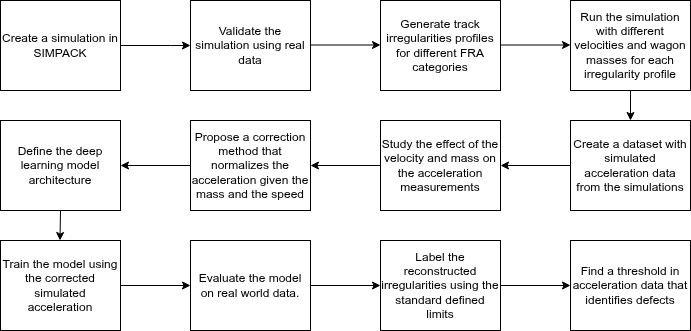
\includegraphics[width=12cm]{Cap3_Methodology/Flowchart/Flowchart.png}
    \caption{Flowchart of the proposed methodology.}
    \label{fig:flowchart}
\end{figure}

\chapter{Results} \label{sec-Results}
